\documentclass{article}

\usepackage{graphicx}
\usepackage{wrapfig}
\usepackage{subcaption}
\usepackage[margin=1in]{geometry}
\usepackage{amsmath} % or simply amstext
\usepackage{amssymb}
\usepackage{siunitx}
\usepackage{booktabs}
\usepackage[export]{adjustbox}
\newcommand{\angstrom}{\textup{\AA}}
\newcommand{\colormap}{jet}  % colorbar to use
\usepackage{cleveref}
\usepackage{booktabs}
\usepackage{gensymb}
\usepackage{float}
\usepackage{xr}

\externaldocument[M-]{Draft}

\title{Supporting Information: Statistical Inference of Transport Mechanisms and Long Time Scale Behavior from Time Series 
       of Solute Trajectories in Nanostructured Membranes.}

\author{Benjamin J. Coscia, Christopher P. Calderon \and Michael R. Shirts} 

\renewcommand{\thefigure}{S\arabic{figure}}
\renewcommand{\thesection}{S\arabic{section}}
\renewcommand{\thepage}{S\arabic{page}}
\renewcommand{\thetable}{S\arabic{table}}

\begin{document}

  \graphicspath{{./supporting_figures/}}
  \maketitle
  
  \section{Parameter Convergence}\label{section:convergence}
  
  The state sequence appears to converge within 500--1000 IHMM iterations. Step 1
  in the procedure from the previous section is the only time the state sequence 
  is determined. We ran 2000 iterations of the IHMM algorithm in order to arrive
  at a finalized state sequence. Stabilization of the VAR parameters indicates 
  that the state sequence has converged. In Figure~\ref{fig:convergence3d}, we plot
  the diagonal entries of 3 different $A$ and $\Sigma$ matrices as well as the 
  entries of the mean vector $\mathbf{c}$, fit to a single 3D methanol trajectory.
  States with a relatively small number of observations are more highly influenced 
  by the boundaries of the state segments and generally lead to much higher 
  variance of the $A$ and $\Sigma$ parameters. In these cases, the mean is
  a more reliable indicator of convergence since stabilized means imply that the
  fluctuations assigned to each state come from motion about a static location.
  
  \begin{figure}[h]
  \centering
  \begin{subfigure}{0.8\textwidth}
  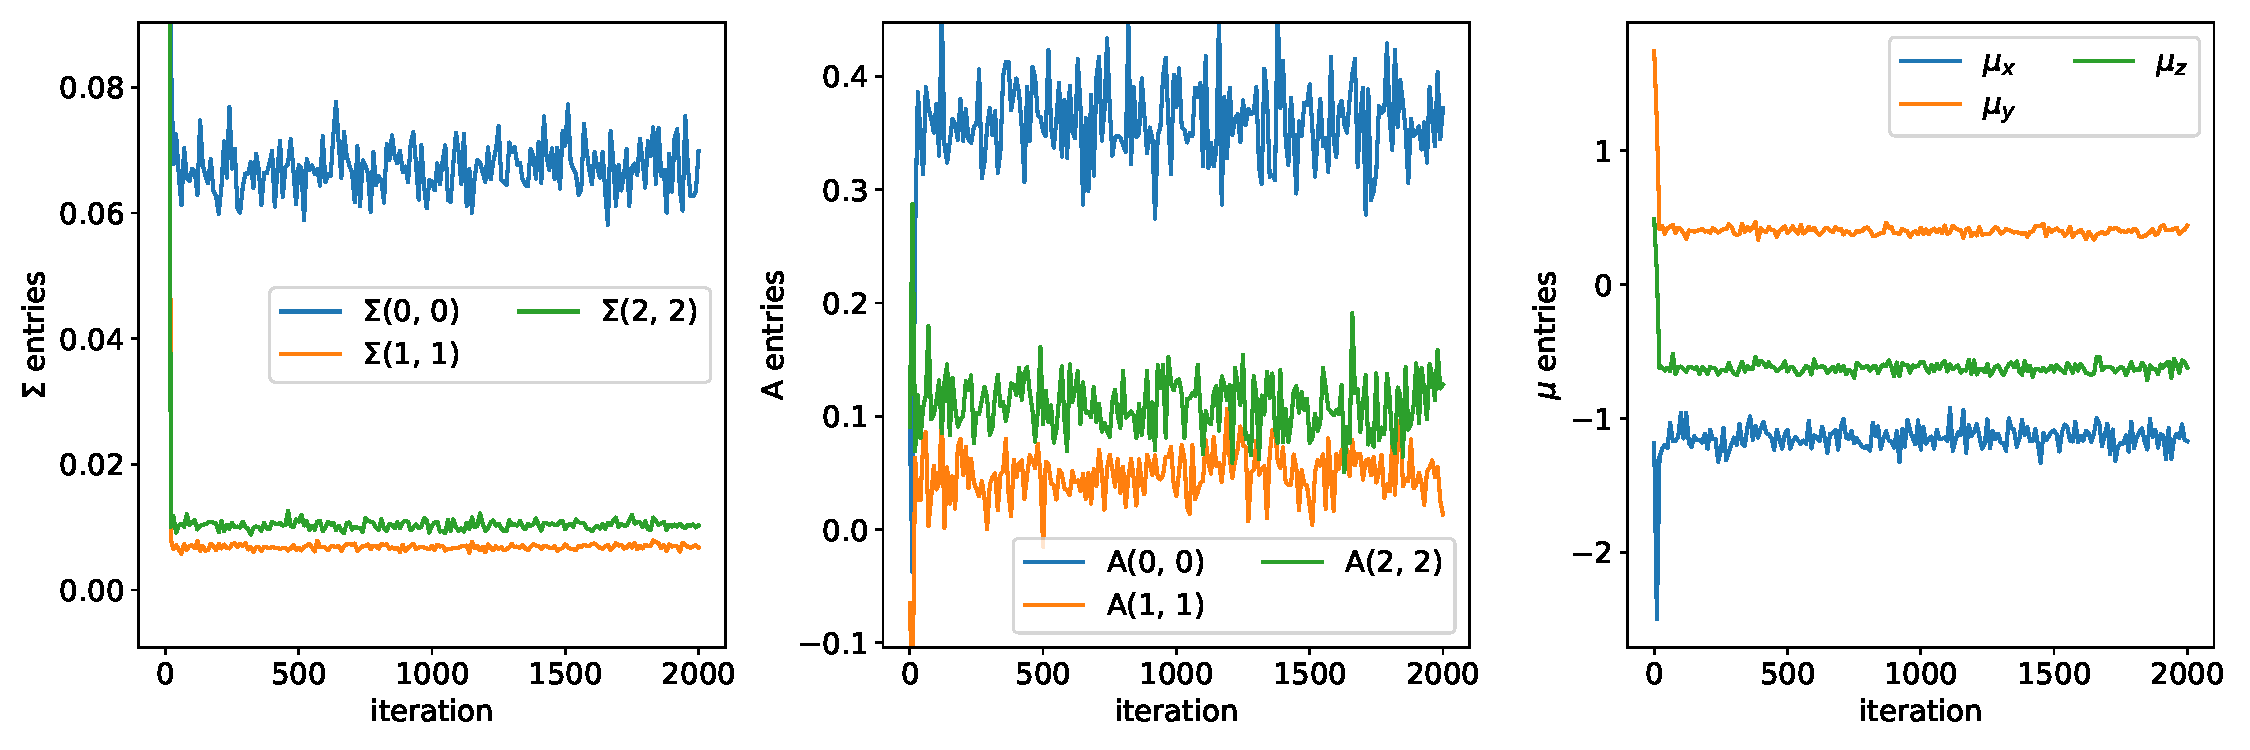
\includegraphics[width=\textwidth]{convergence_MET_47.pdf}
  \caption{706 total emissions}\label{fig:convergence3d_MET_low}
  \end{subfigure}
  \begin{subfigure}{0.8\textwidth}
  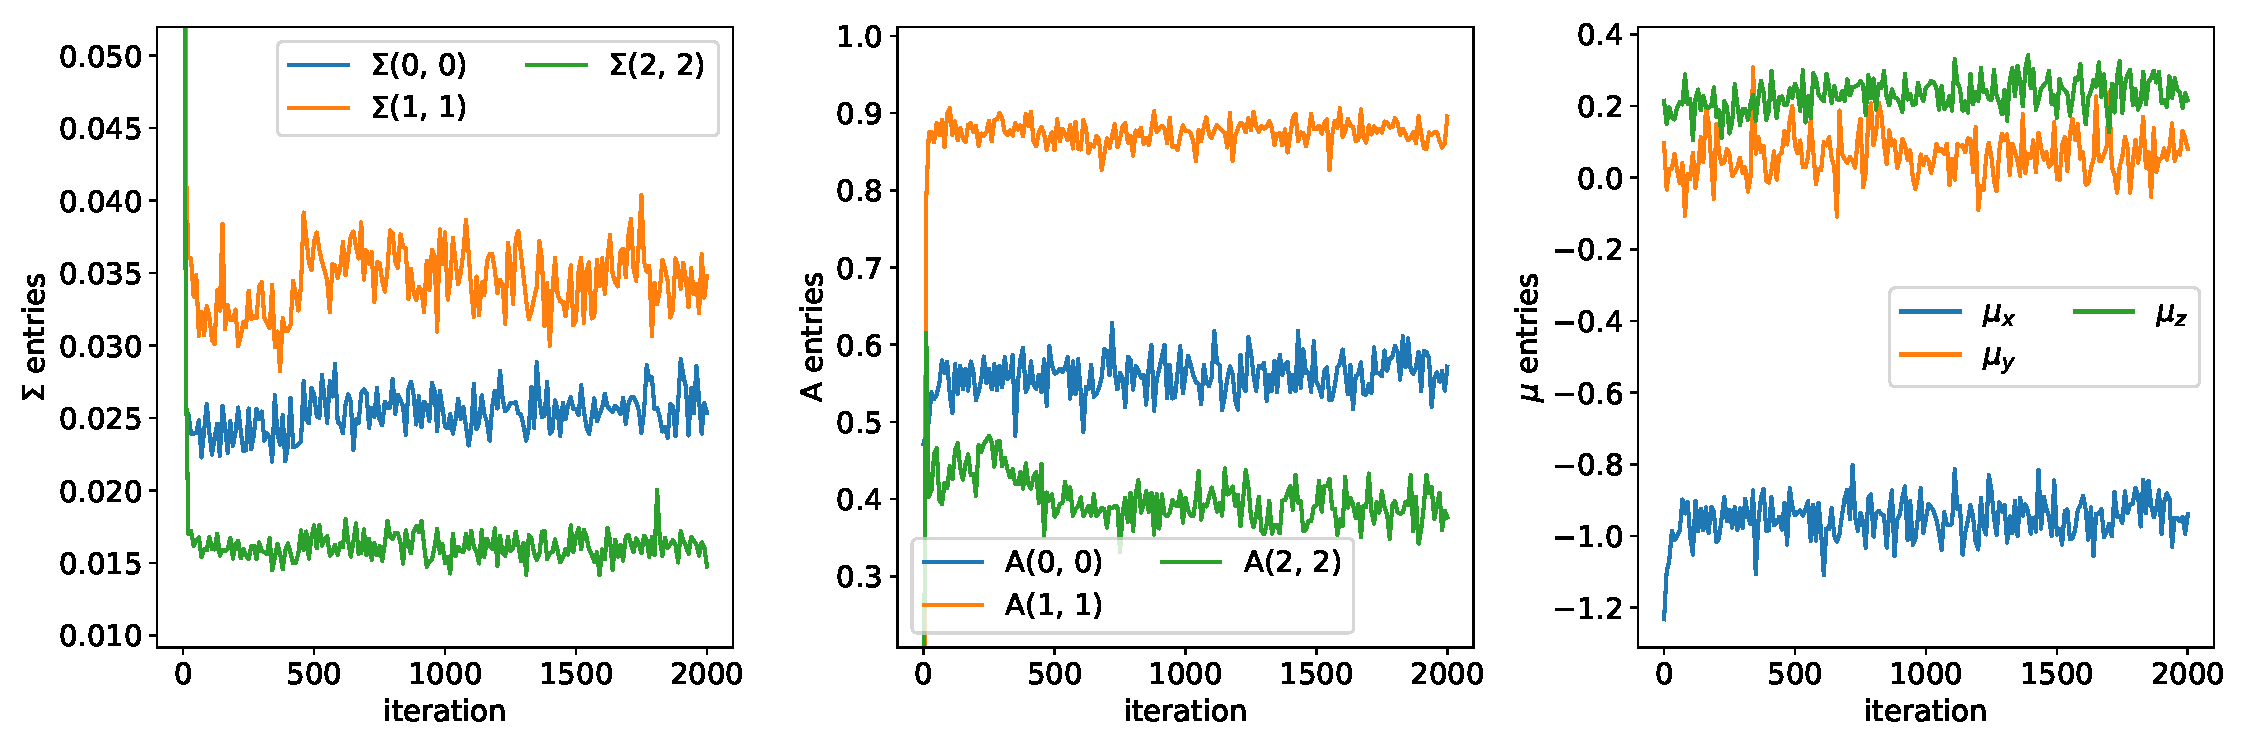
\includegraphics[width=\textwidth]{convergence_MET_36.pdf}
  \caption{1000 total emissions}\label{fig:convergence3d_MET_medium}
  \end{subfigure}
  \begin{subfigure}{0.8\textwidth}
  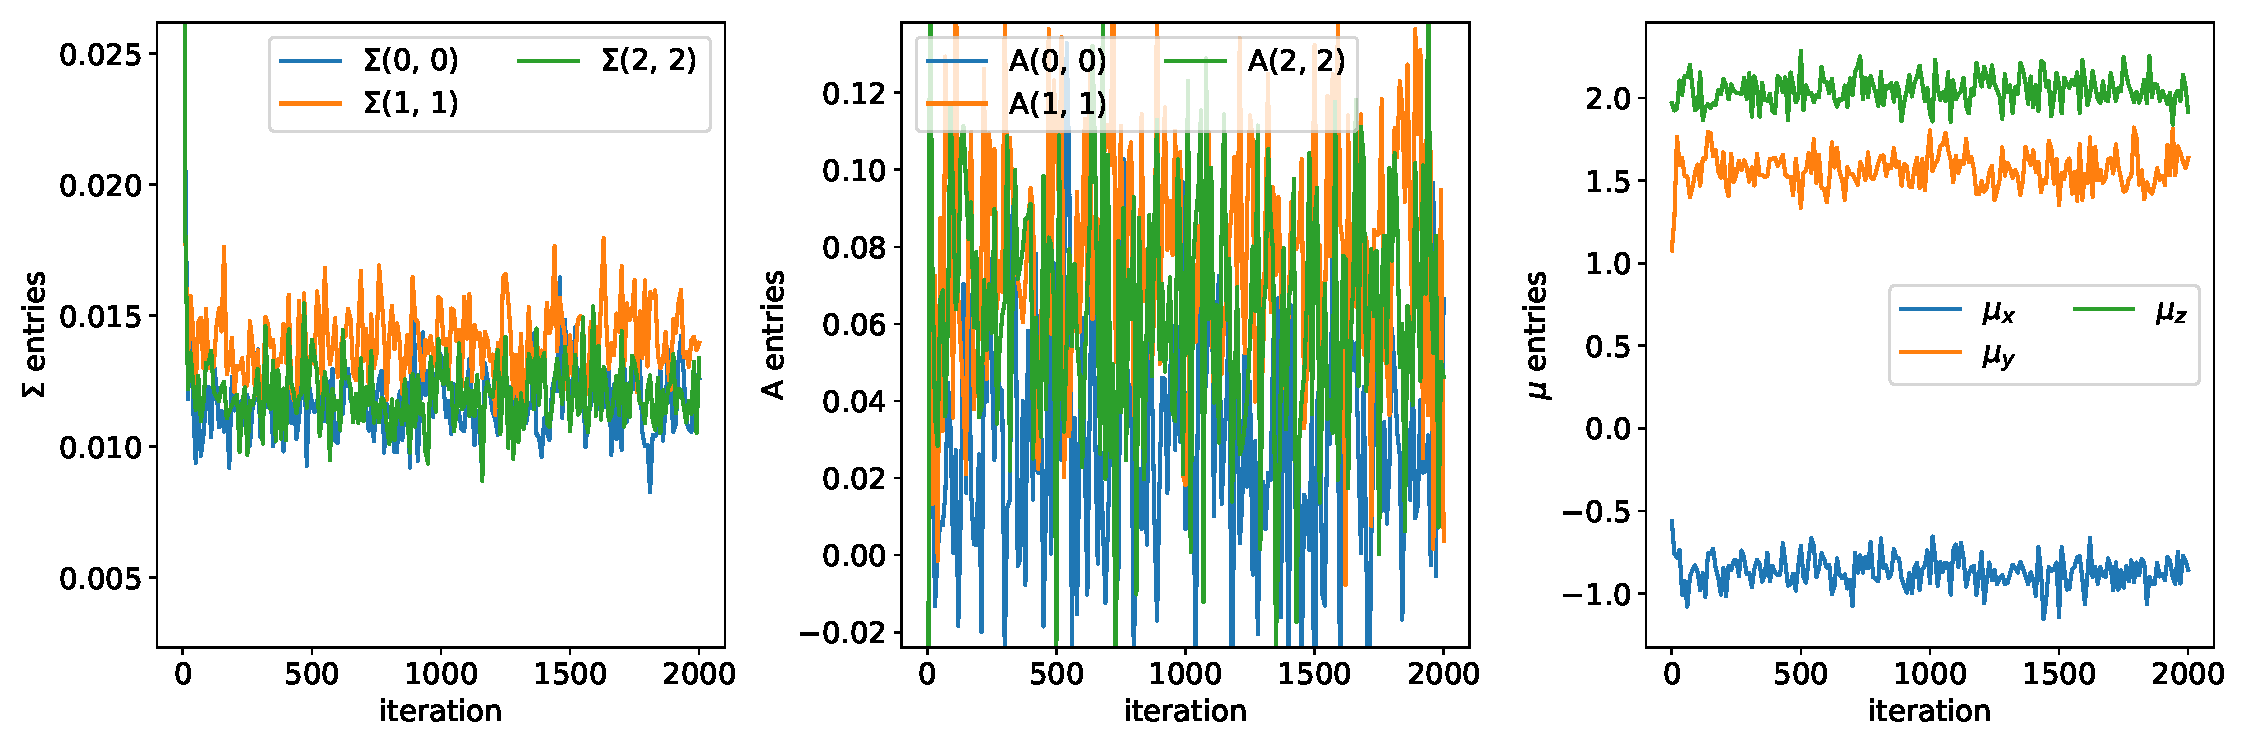
\includegraphics[width=\textwidth]{convergence_MET_59.pdf}
  \caption{201 total emissions}\label{fig:convergence3d_MET_high}
  \end{subfigure}
  \caption{Given a sufficient number of observations for a given mode, the VAR parameters
  appear to converge within 500 -- 1000 iterations. States with too few observations
  are more highly influenced by the boundaries of the state segments and generally
  lead to much higher fluctuations in the VAR parameters.}\label{fig:convergence3d}
  \end{figure}
  
  \clearpage
  
  When we fix the state sequence in subsequent steps of the procedure, parameter 
  estimates converge within only a few steps. In Figure~\ref{fig:fixed_state_convergence}, we 
  plot the entries of $A$ and $\Sigma$ as a function of IHMM iteration. Some states
  are sampled far more frequently than others. High sampling frequently results in
  higher certainty converged parameter estimates. Due to fast convergence, we only
  run 100 iterations of the inference behavior when the state sequence is fixed.
  
  \begin{figure}[h]
  \centering
  \begin{subfigure}{0.6\textwidth}
  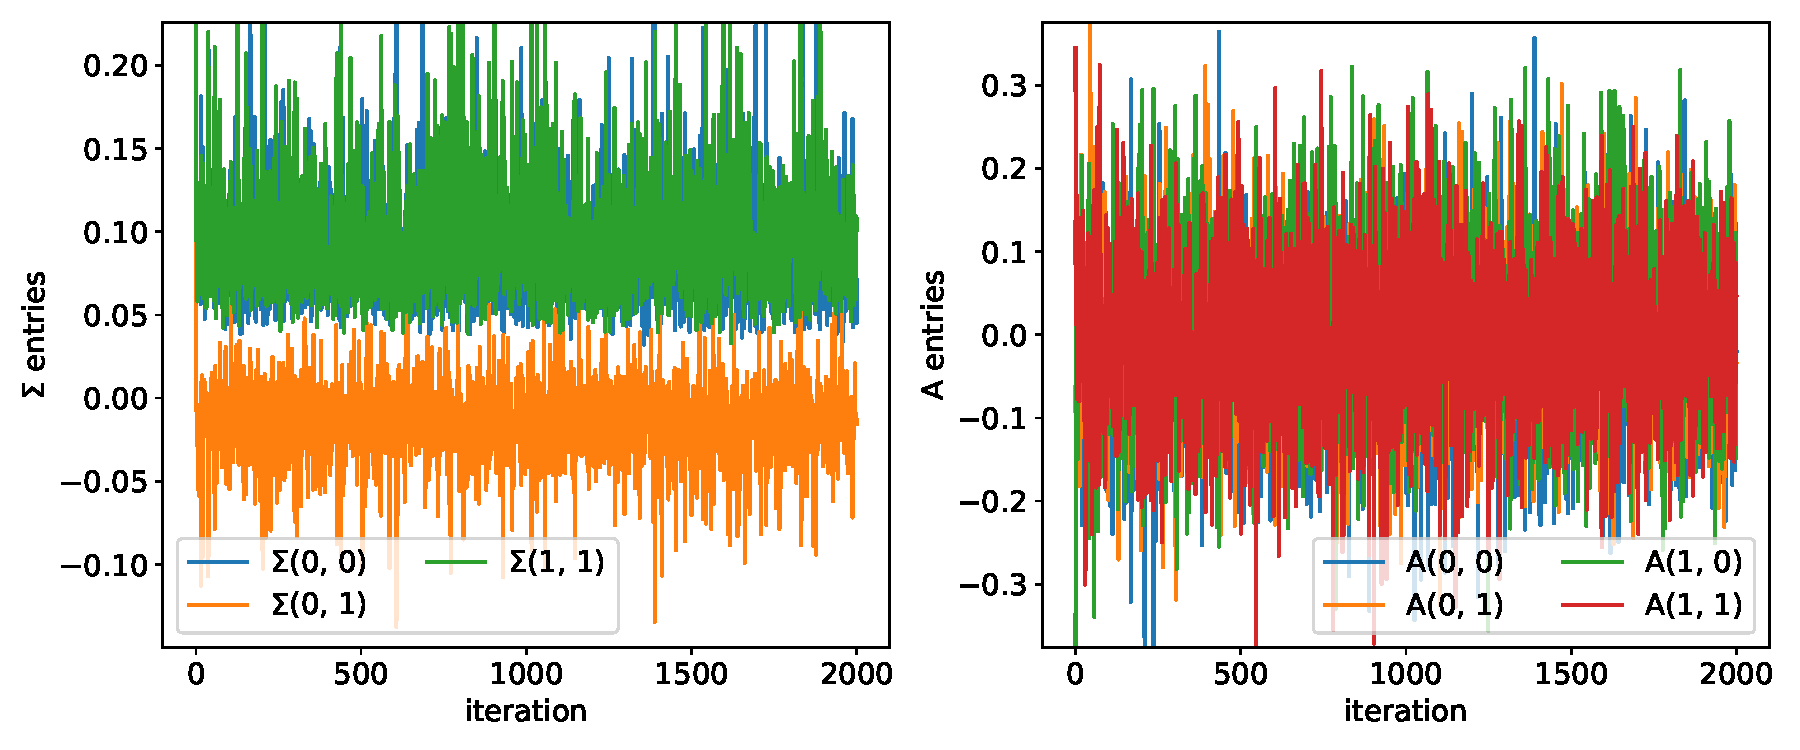
\includegraphics[width=\textwidth]{convergence_MET_4.pdf}
  \caption{15 total emissions}\label{fig:convergence_MET_low}
  \end{subfigure}
  \begin{subfigure}{0.6\textwidth}
  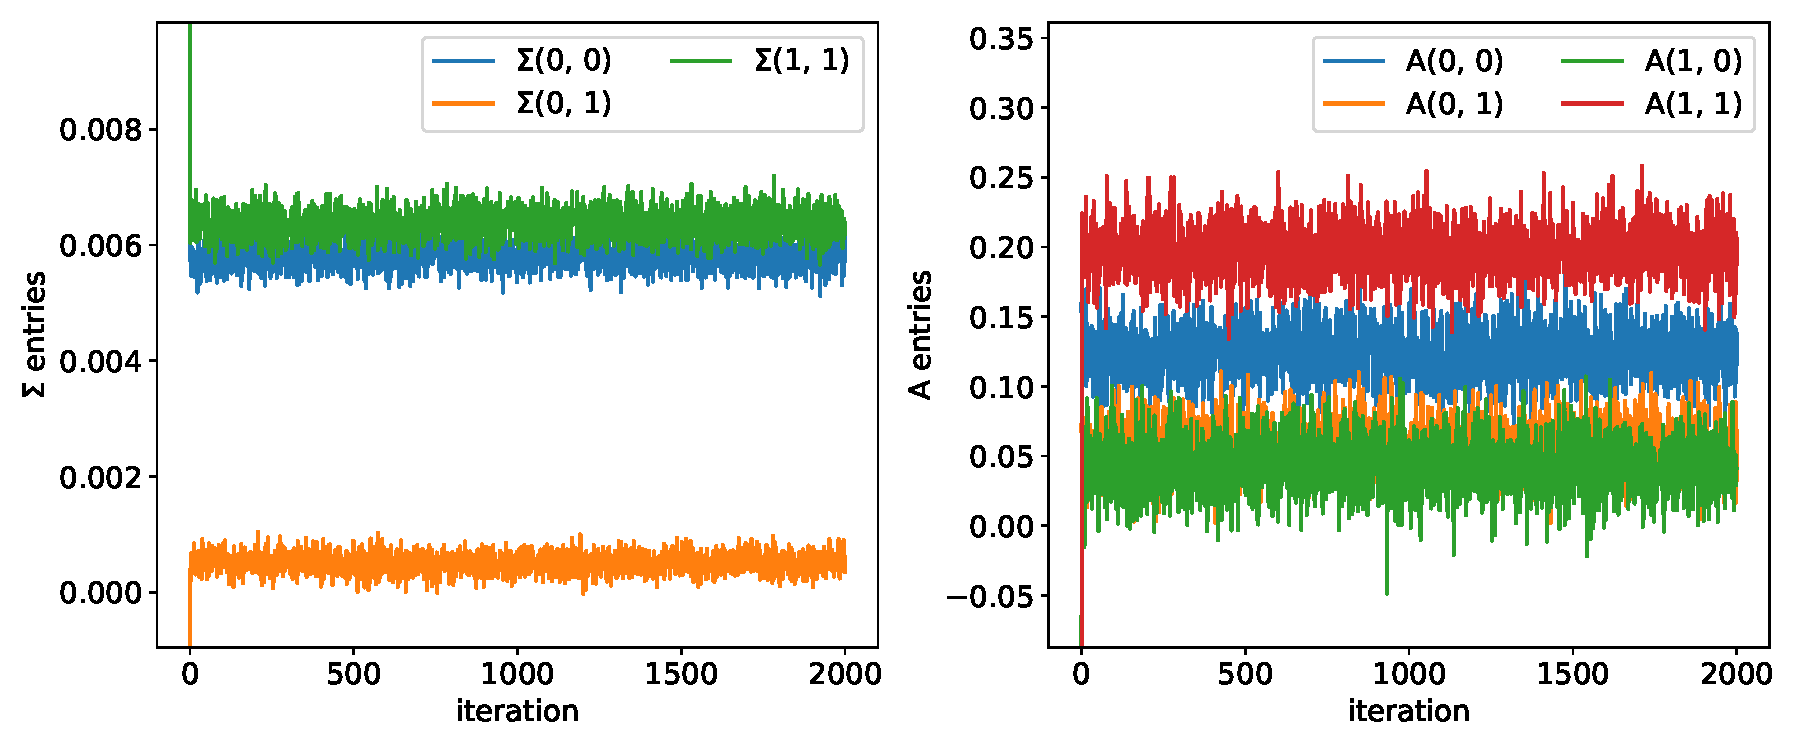
\includegraphics[width=\textwidth]{convergence_MET_21.pdf}
  \caption{1289 total emissions}\label{fig:convergence_MET_medium}
  \end{subfigure}
  \begin{subfigure}{0.6\textwidth}
  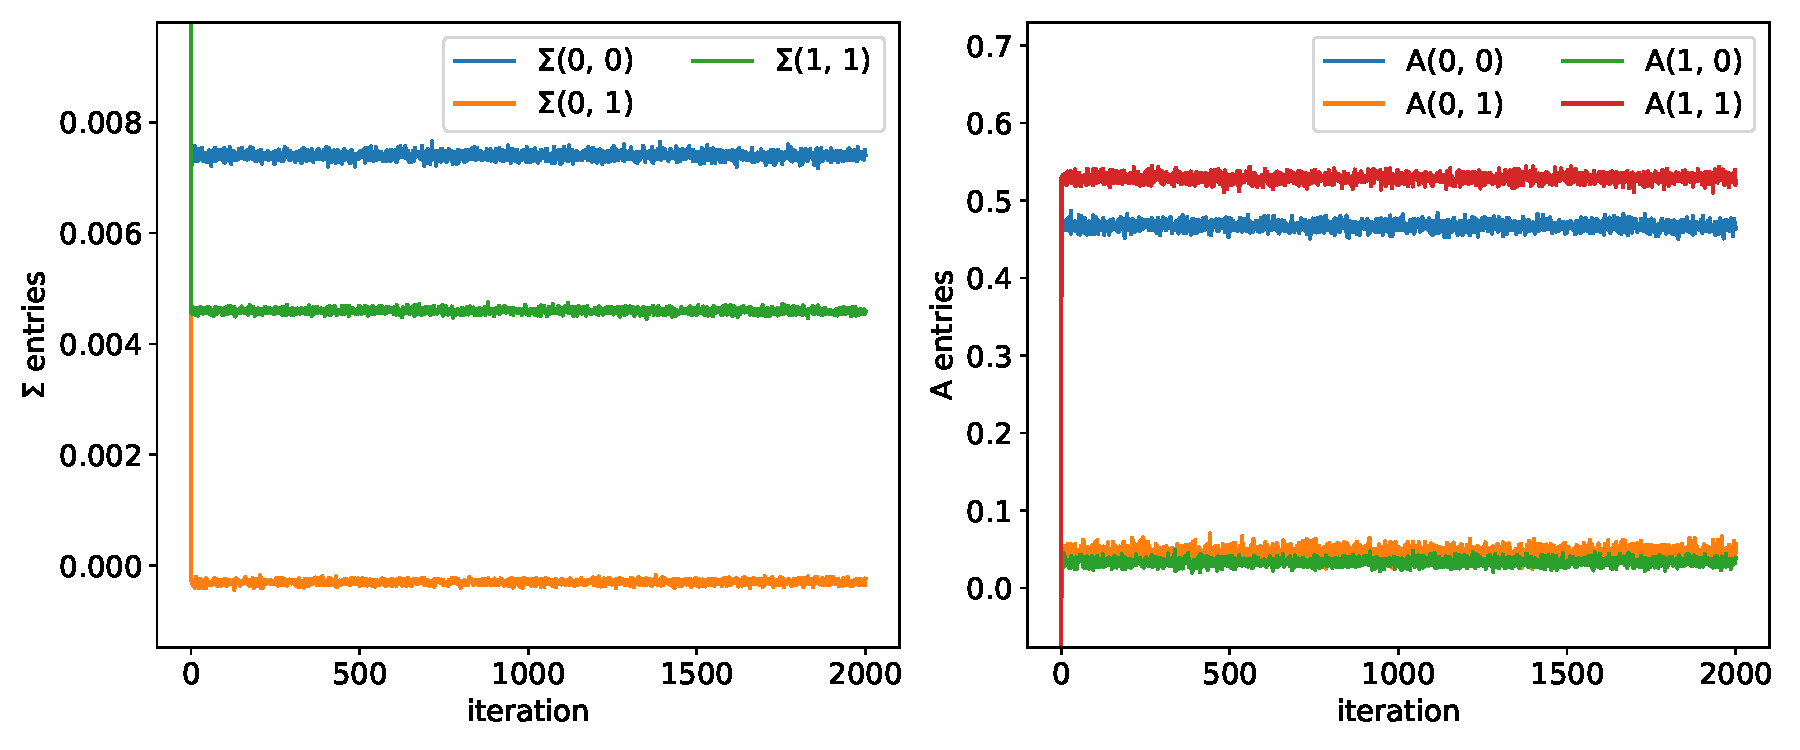
\includegraphics[width=\textwidth]{convergence_MET_15.pdf}
  \caption{24468 total emissions}\label{fig:convergence_MET_high}
  \end{subfigure}
  \caption{The VAR parameters converge quickly when we fix the state
  sequence. As the total number of emissions observed from each state
  increases, the uncertainty in the converged parameters estimates
  decreases.}\label{fig:fixed_state_convergence}
  \end{figure}
  
  \clearpage
  
  \section{Demonstration of IHMM Parameterization Procedure}\label{section:ihmm_procedure}
  
  Parameterization of trajectories by the IHMM is a multi-stepped procedure. In the steps and
  figures that follow, we graphically illustrate the procedure which is described in detail 
  in Section~\ref{M-method:IHMM} of the main text.
  
  \begin{enumerate}
  	\item Parameterize in $x$, $y$, $z$ coordinates with $x$, $y$ coordinates relative to the nearest
  	pore center (see Figure~\ref{fig:xyz_hmm}). 		
  	\item Cluster the VAR parameters from the states found in all 24 trajectories (See 
  	Section~\ref{method:clustering} of the main text). Reassign the state sequence so that segments
  	which belong to the same cluster are labeled the same across all solute trajectories.
  	\item Zero the trajectories. First, zero out the $y$ dimension by rotating each segment of 
  	the trajectory, as partitioned before clustering, about the $z$ axis, in order to align the 
  	mean $xy$ vector with the $x$ axis (see Figure~\ref{fig:y_zeroed}). Then, subtract the mean in
  	$x$ and $z$ (Figure~\ref{fig:xyz_zeroed}.
  	\item Fix clustered state sequence and infer parameters of each state, assuming a mean of zero
  	for all states (see Figure~\ref{fig:zeroed_clustered_hmm}). 
  \end{enumerate}
  
  \begin{figure}
    \centering
	\begin{subfigure}{0.6\textwidth}
	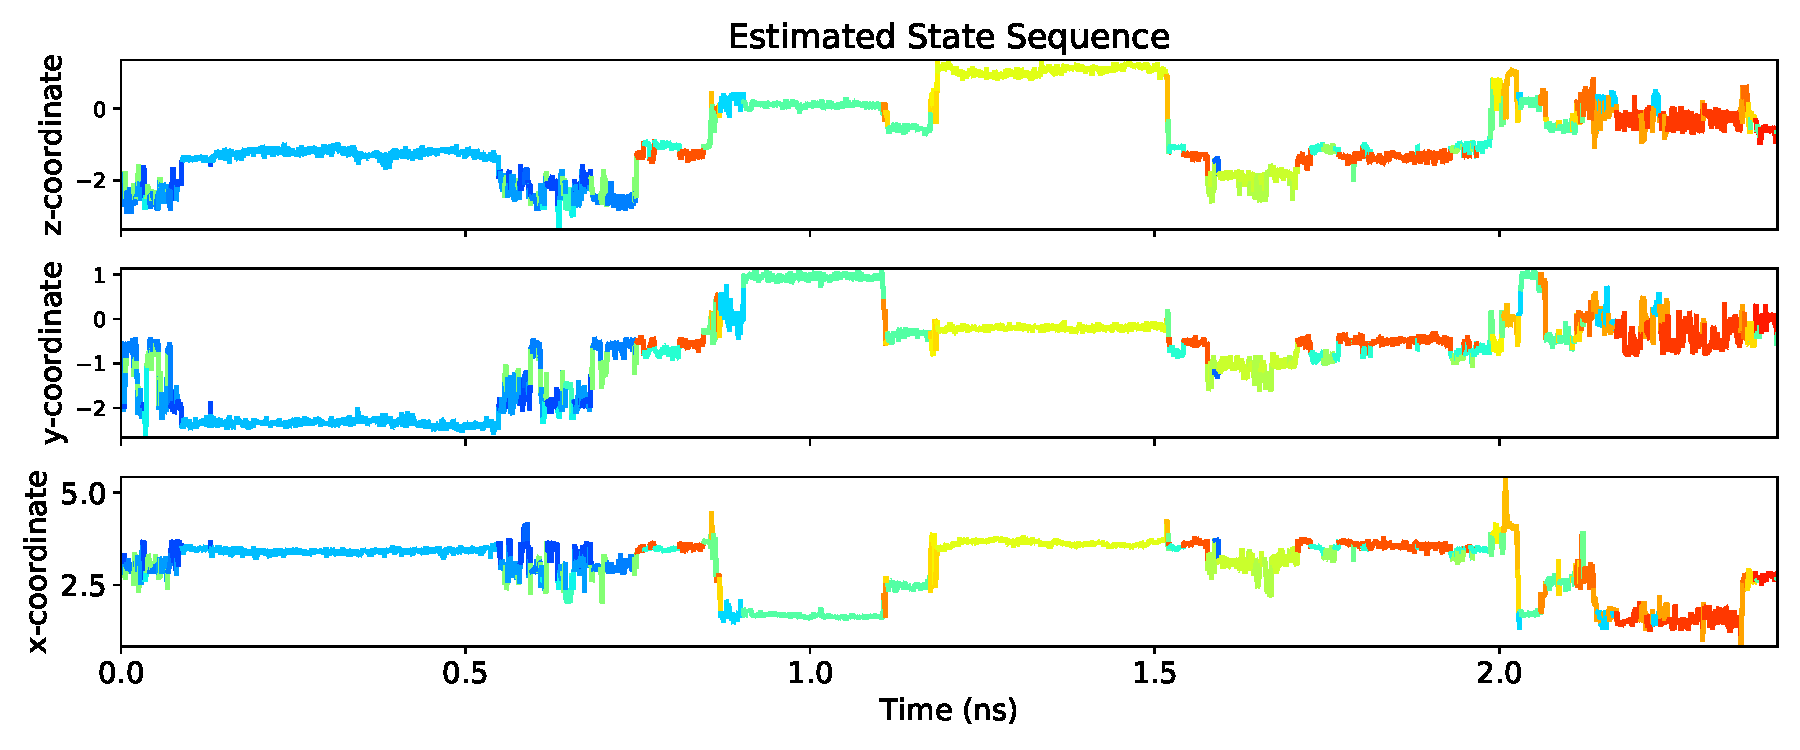
\includegraphics[width=\textwidth]{xyz_hmm.pdf}
		\caption{}\label{fig:xyz_hmm}
	\end{subfigure}  
		\begin{subfigure}{0.6\textwidth}
		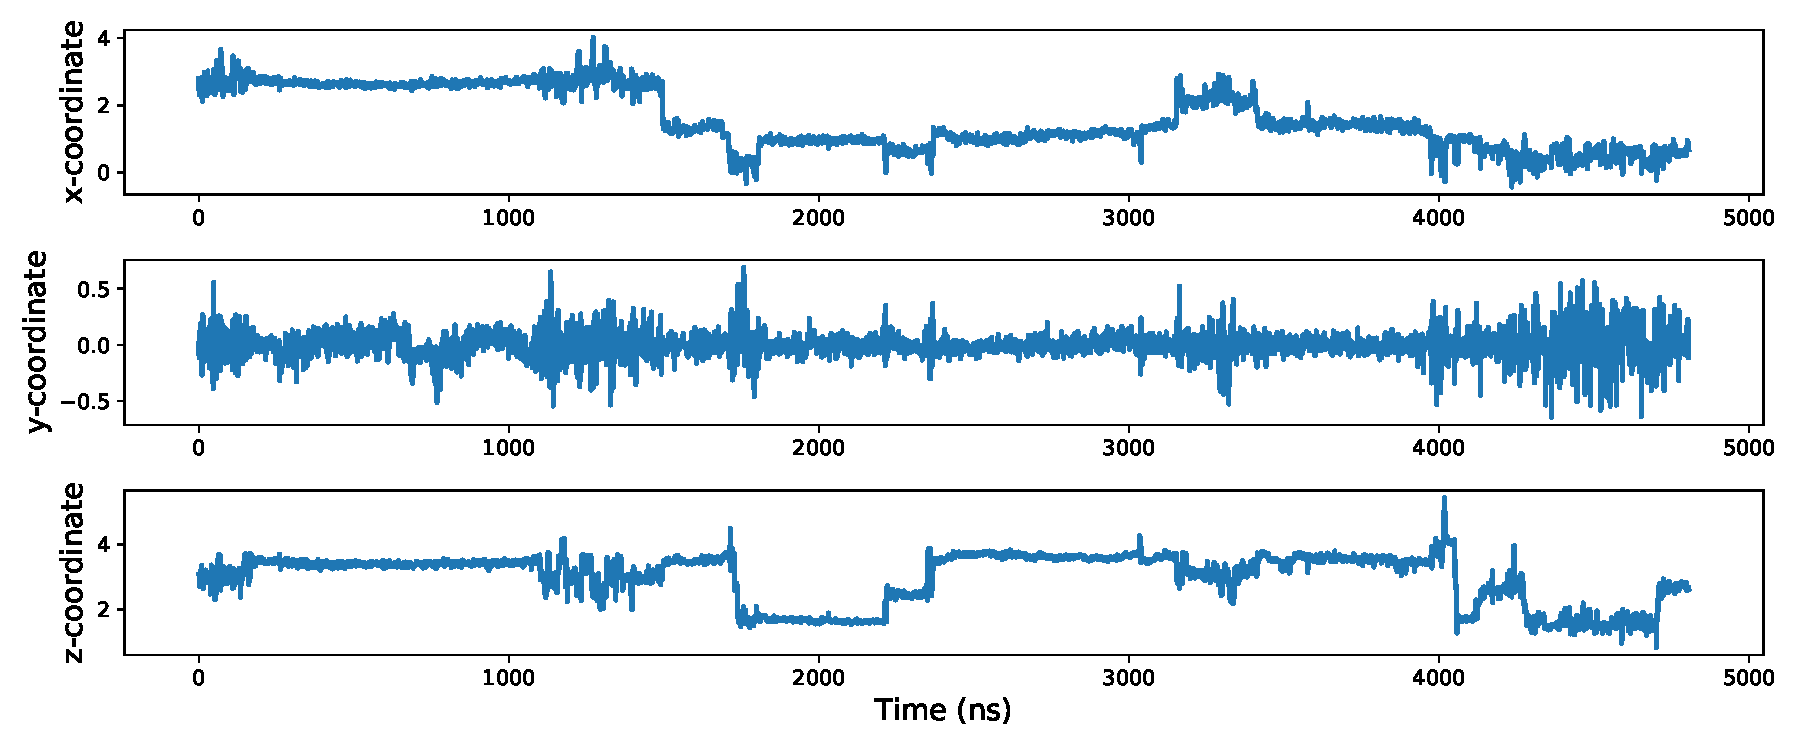
\includegraphics[width=\textwidth]{y_zeroed.pdf}
		\caption{}\label{fig:y_zeroed}
	\end{subfigure}  	
	\begin{subfigure}{0.6\textwidth}
		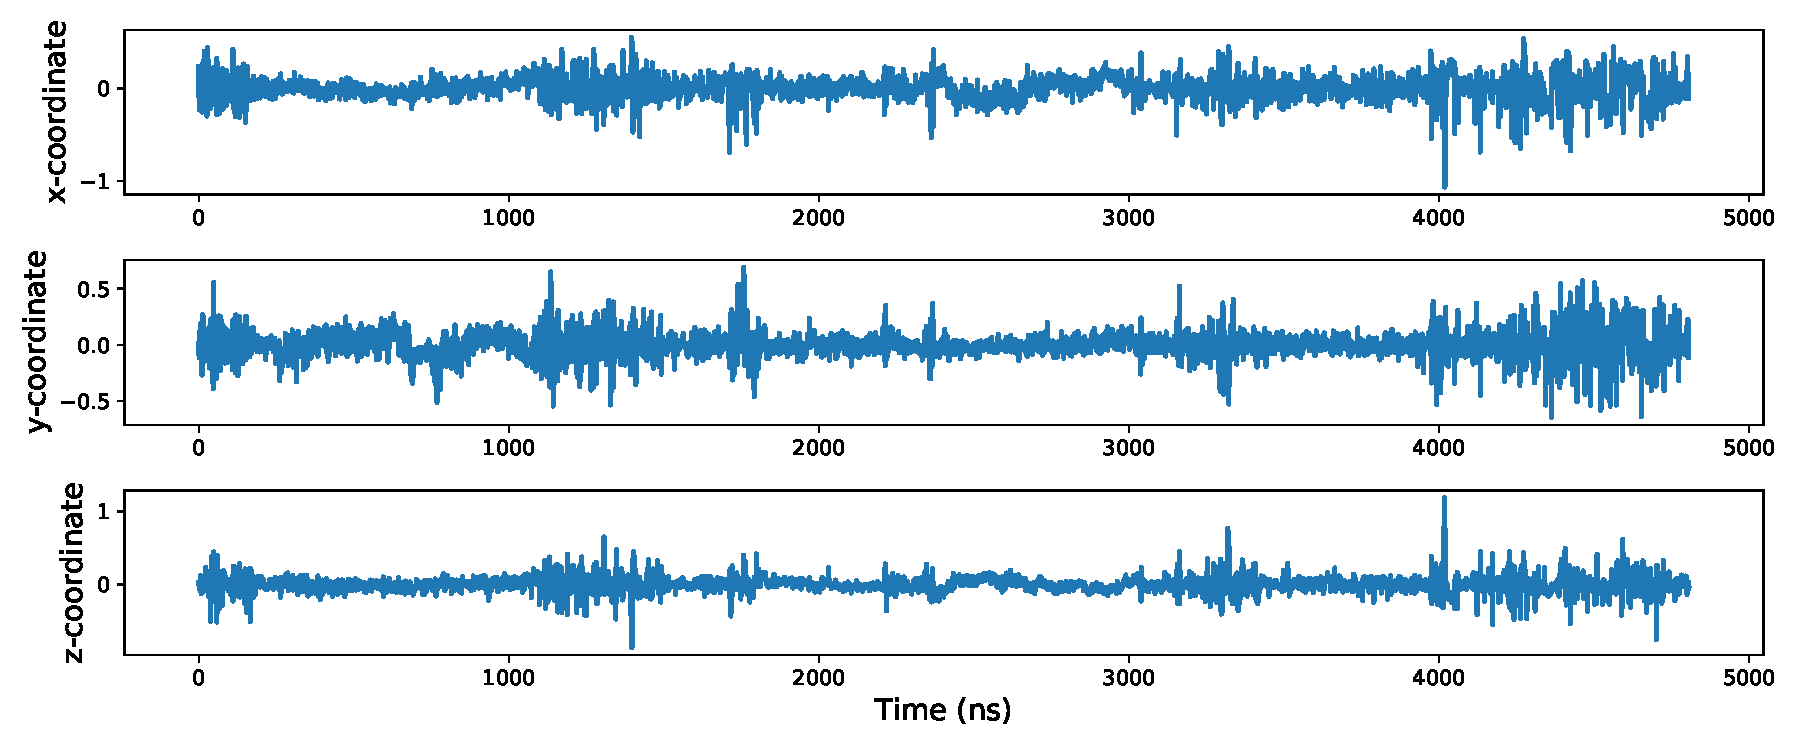
\includegraphics[width=\textwidth]{xyz_zeroed.pdf}
		\caption{}\label{fig:xyz_zeroed}
	\end{subfigure}  		
	\begin{subfigure}{0.6\textwidth}
		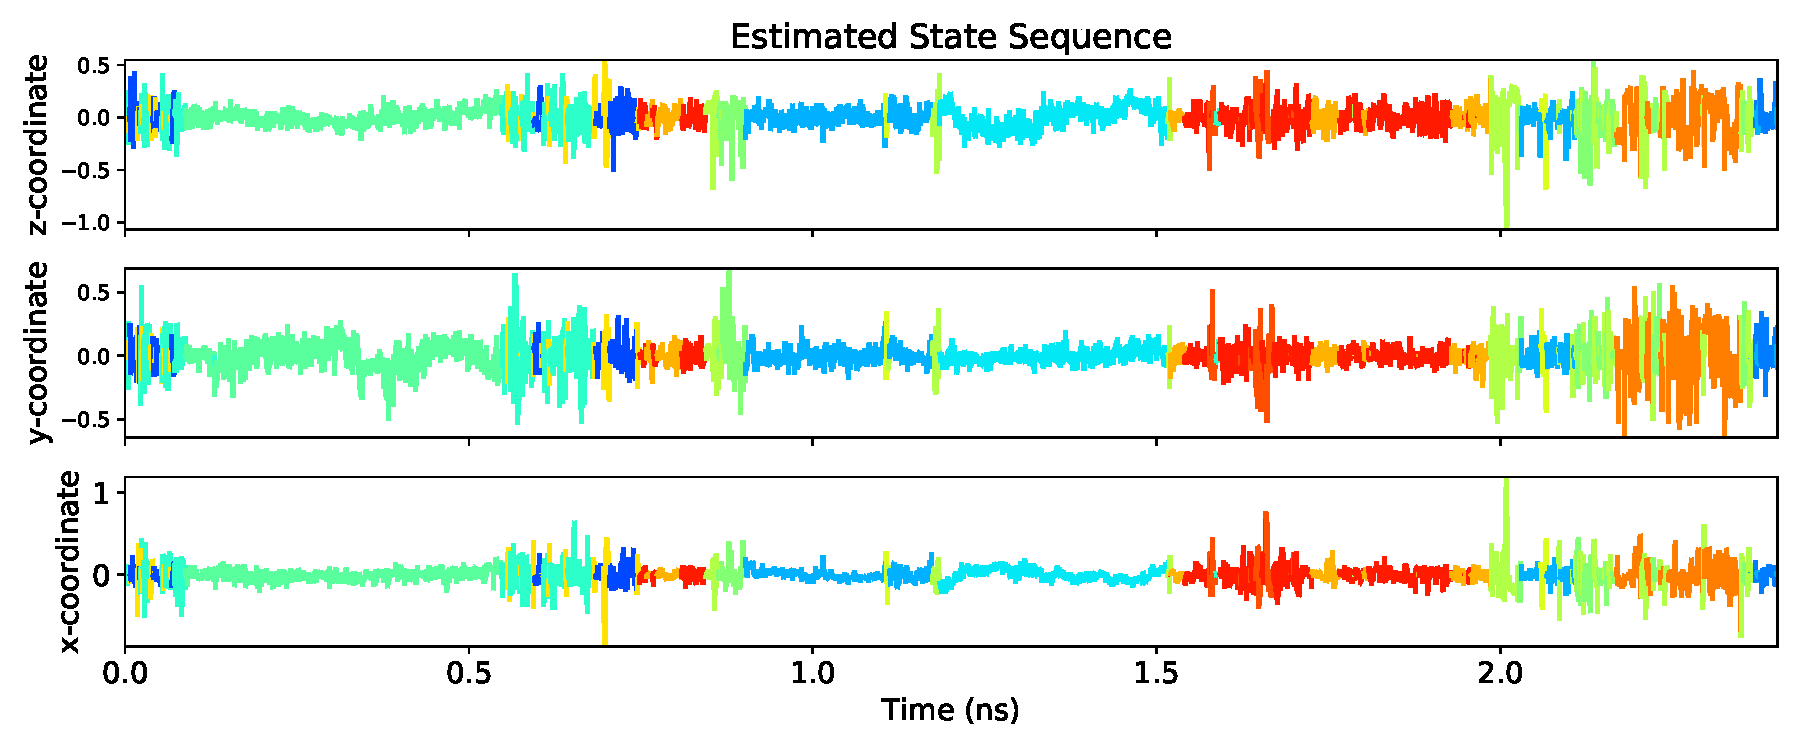
\includegraphics[width=\textwidth]{zeroed_clustered_hmm.pdf}
		\caption{}\label{fig:zeroed_clustered_hmm}
	\end{subfigure}  
	\caption{IHMM parameterization is a multi-step procedure. In the above plots, distinct colors
	correspond to distinct state behavior. (a) First we parameterize the trajectories in terms of
	the $x$, $y$, $z$ solute center-of-mass coordinates with the $x$ and $y$ coordinates relative
	to the nearest pore center (b) Next, we convert the $x$ and $y$ 	
	coordinates to radial coordinates, $r$, then fix the state sequence and use the inference 
	component of the IHMM in order to estimate the parameters in terms of $r$ and $z$. Note that
	the segment colors in (b) are the same as (a) because we fixed the state sequence.
	(c) After clustering the VAR parameters and reassigning the state sequence so that segments 
	which belong to the same cluster are labeled the same across all solute trajectories, we subtract
	the mean of each segment, obtained before clustering, in order to zero out the
  	trajectory, and then fix the clustered state sequence to infer the parameters of each clustered 
  	state, assuming a mean of zero for all states. Note that the colors are no longer aligned with 
  	figures (a) and (b) because the states are relabeled in terms of their clusters. There are
  	also less states in this single trajectory.
	}\label{fig:hmm_demo}
  \end{figure}
  
  \newpage
    
  \section{Tips for Reliable State Sequence Identification}\label{section:fitting_tips}
  
  \textit{Choosing Prior Parameters}: The states identified by the IHMM are 
  heavily influenced by the Gaussian prior placed on $\mathbf{c}$ in 
  Equation~\ref{M-eqn:var} of the main text. The entries of $A$ and $\Sigma$
  do not vary over a wide range, so the final parameters were relatively 
  insensitive to the priors. In order to maximally automate the IHMM procedure,
  we attempted to parameterize the
  prior on $\mathbf{c}$ in an intelligent way. The prior parameters should
  be chosen such that the mean level of each state lies within a region of 
  reasonable probability of the prior (see Figure~\ref{fig:prior_guesses}).
  In each dimension, we defined the prior mean to lie halfway between the 
  maximum and minimum of each trajectory dimension. To parameterize the 
  prior's variance in each dimension, we defined the maximum and minimum to 
  be 2 standard deviations from the prior mean. Although this approach has 
  worked quite well for the data in this work, it is important to check the 
  results to determine whether further adjustments to the prior might be needed.
%  In Figure TBD, we show the result of a parameterization where the prior
%  parameters of $c$ were poorly chosen. %TODO
  
  \begin{figure}[h]
  \centering
  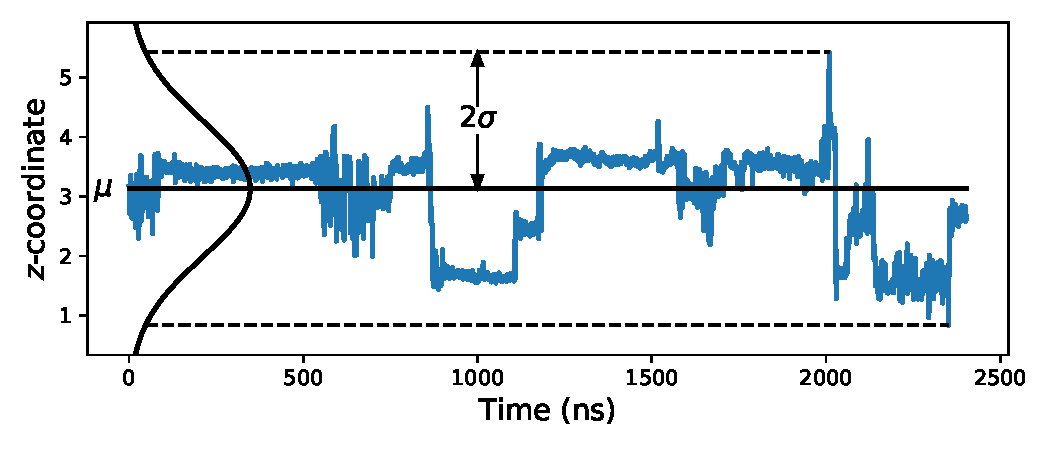
\includegraphics[width=\textwidth]{prior_guesses.pdf}
  \caption{The parameters of the prior on the mean vector, $\mathbf{c}$, (black line), which
  represents the coordinates at which solute are trapped, should be chosen such
  that the mean levels of each state identified in the trajectory (blue line) lie within
  regions of the prior with reasonable probability. We chose the mean of the prior 
  as halfway between the maximum and minimum (shown by the dashed lines) of each trajectory dimension. We chose 
  $\sigma$ of the prior by defining the maximum and minimum to be 2 standard deviations
  from the mean.}\label{fig:prior_guesses}
  \end{figure}
  
  \pagebreak
  
  The IHMM is quite powerful on its own, but requires some critical thinking by
  the user in order to ensure maximum effectiveness. One can obtain 
  the best results with some simple checks and, where necessary, improved 
  state sequence initialization.
  
  The best way to ensure reliable MSD predictions is to ensure proper reproduction
  of the individual MD MSDs by realizations of the IHMM. Over-predictions and 
  under-predictions are usually the result of a poorly identified state sequence. (see
  Figure TBD for example)
  
  \begin{figure}
  \centering
  \begin{subfigure}{0.35\textwidth}
  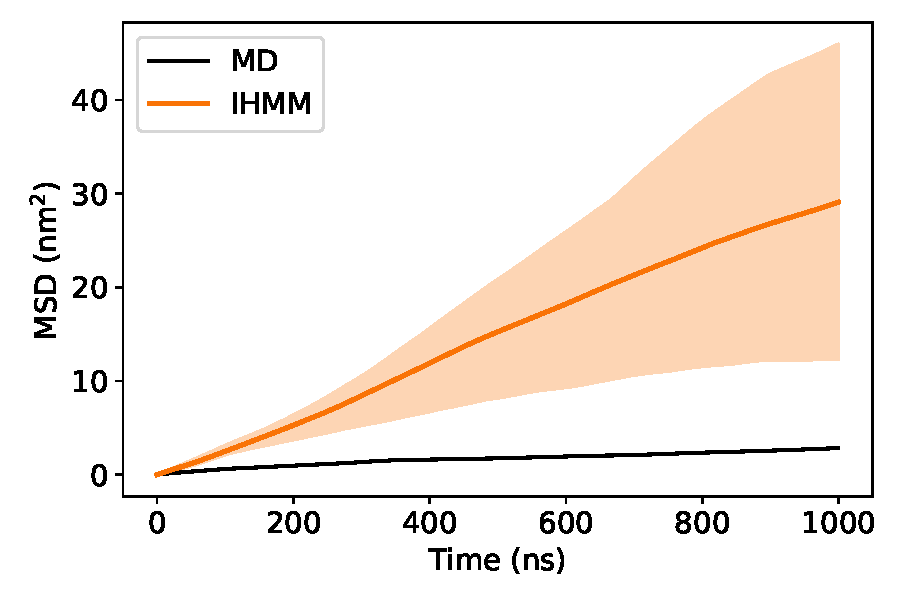
\includegraphics[width=\textwidth]{overestimate_ACH_21.pdf}
  \caption{}\label{fig:msd_overestimate}
  \end{subfigure}
  \begin{subfigure}{0.63\textwidth}
  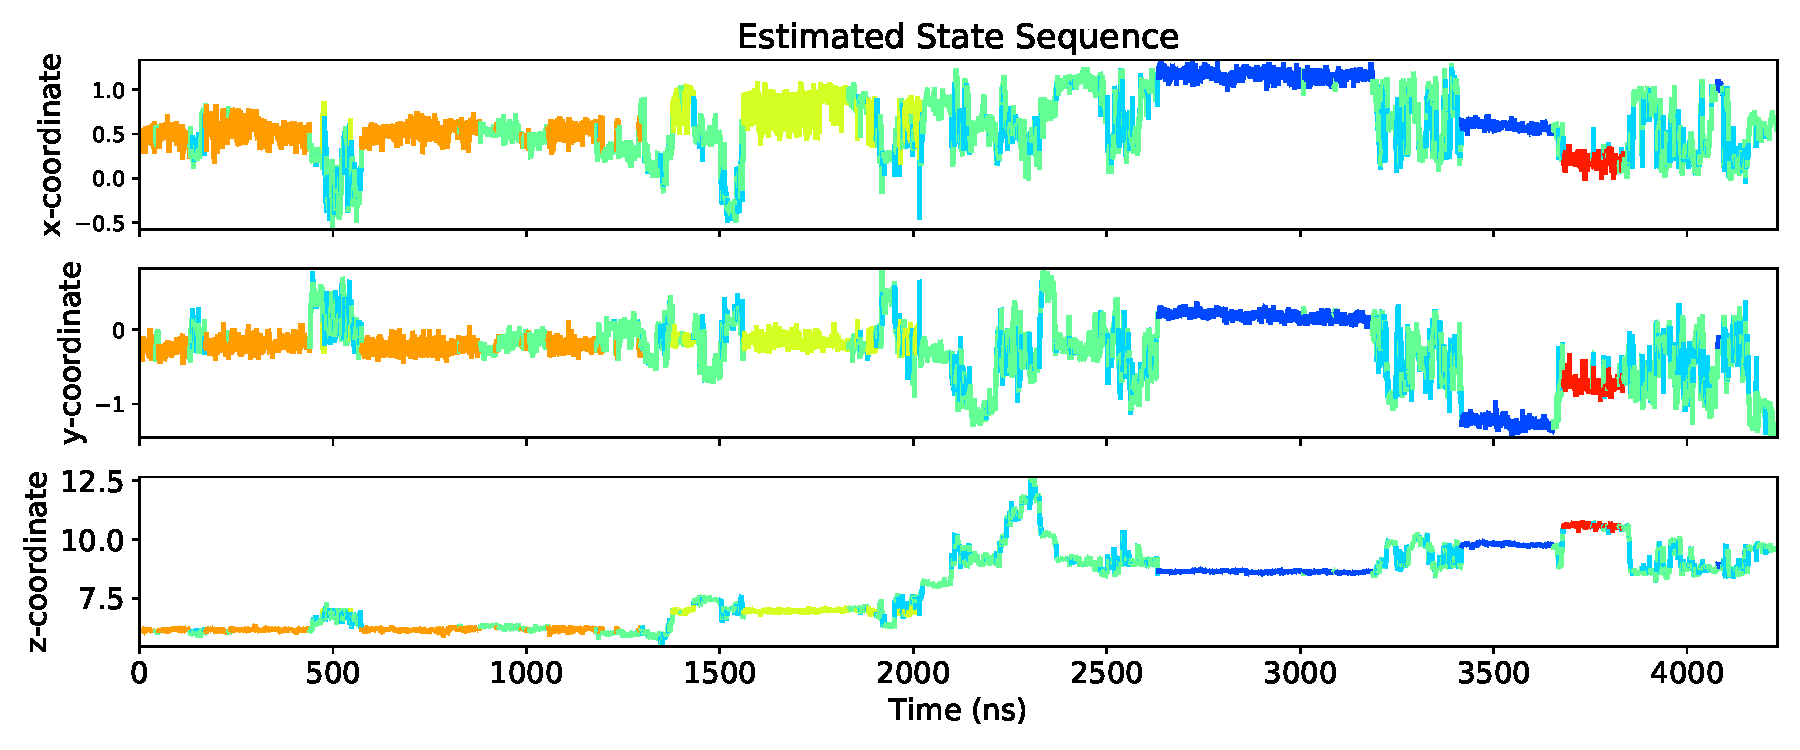
\includegraphics[width=\textwidth]{state_sequence_before_ACH_21.pdf}
  \caption{}\label{fig:state_sequence_before}
  \end{subfigure}
  \begin{subfigure}{0.35\textwidth}
  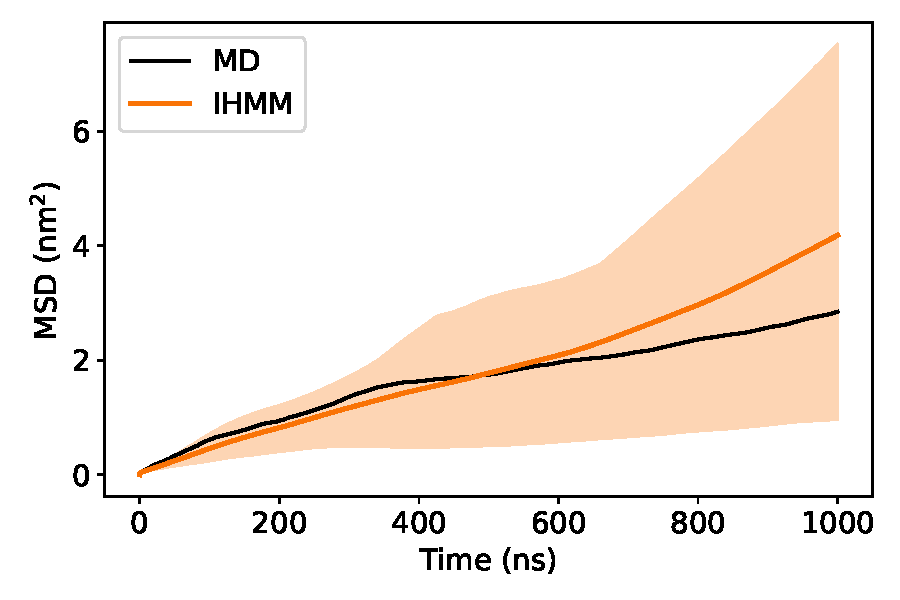
\includegraphics[width=\textwidth]{msd_improvement_ACH_21.pdf}
  \caption{}\label{fig:msd_improvement}
  \end{subfigure}
  \begin{subfigure}{0.63\textwidth}
  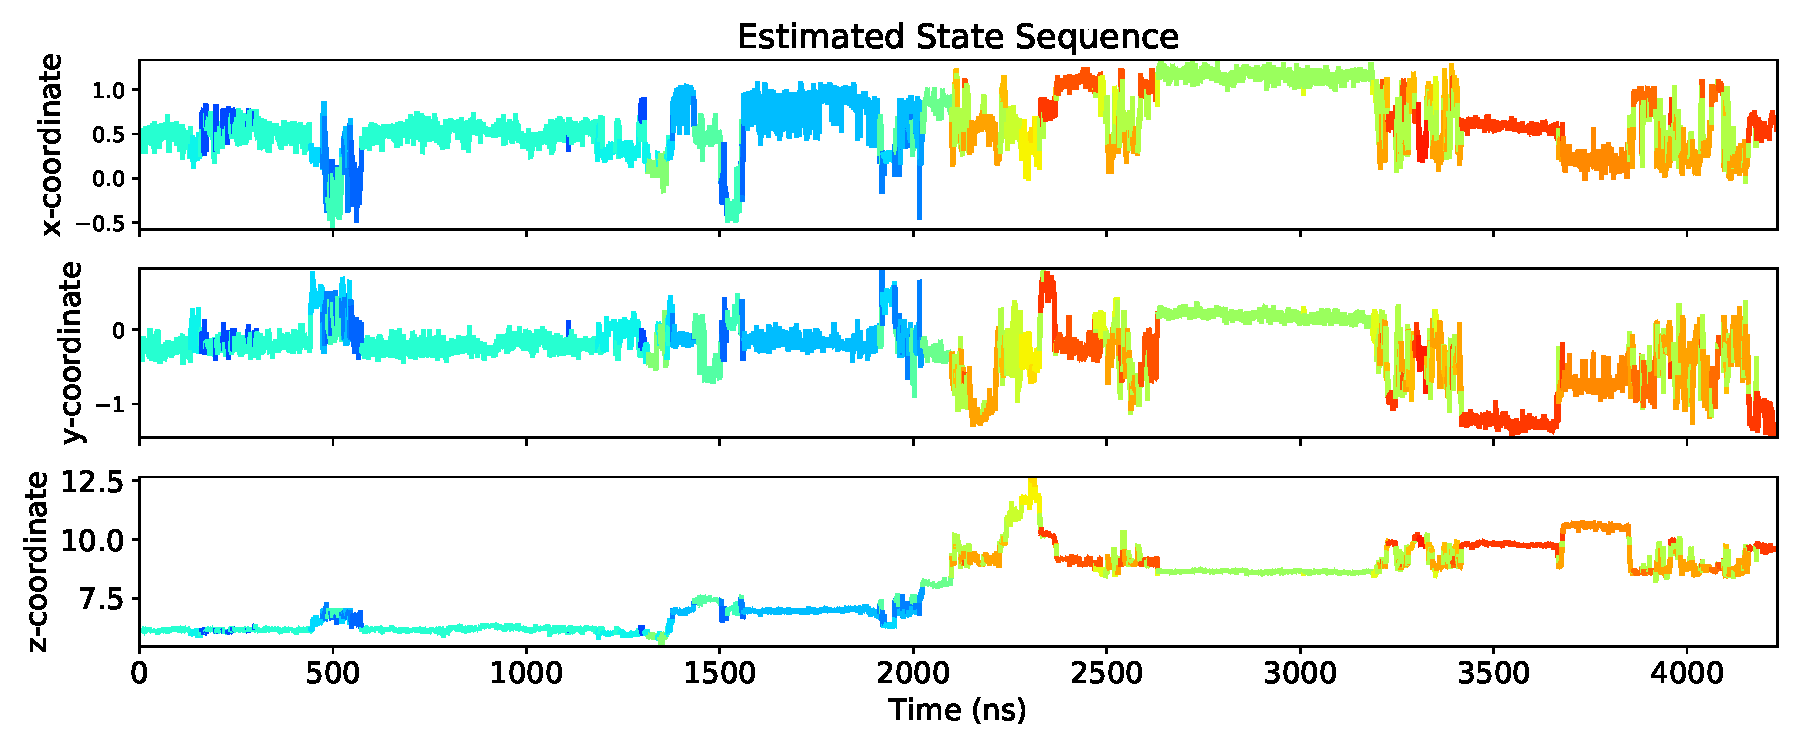
\includegraphics[width=\textwidth]{state_sequence_after_ACH_21.pdf}
  \caption{}\label{fig:state_sequence_after}
  \end{subfigure}
  \caption{(a, b) In some cases, the state segmentation leads to over- or 
  under-prediction of the MSD, usually due to poor initialization of the state
  sequence. In (b), state transitions are too frequent and lead to an
  overprediction of the MD MSD. (c) We can greatly improve MSD predictions by
  giving the IHMM a good guess at the initial state sequence. (d) A better
  initial state segmentation via seeding, gives more reasonable estimates
  of the final state sequence.}\label{fig:improvement_state_sequence}
  \end{figure}
  
  There are two primary approaches we have implemented in order to improve the final 
  state sequence predictions. Both attempt to aid the initial state assignments 
  algorithmically. First, we always initialize the prior on $\mathbf{c}$ in 
  Equation~\ref{M-eqn:var} of the main text as described in 
  Section~\ref{section:prior_guesses}. In particularly tricky cases, the initial
  state sequence estimate is so poor that qualitative trajectory realizations
  and MSD predictions are irreconcilable with MD. In our second approach, we can
  seed the initial state sequence with a guess made by applying the IHMM to 
  smaller segments of the trajectory. 
  
  \begin{figure}
  \centering
  \begin{subfigure}{0.48\textwidth}
  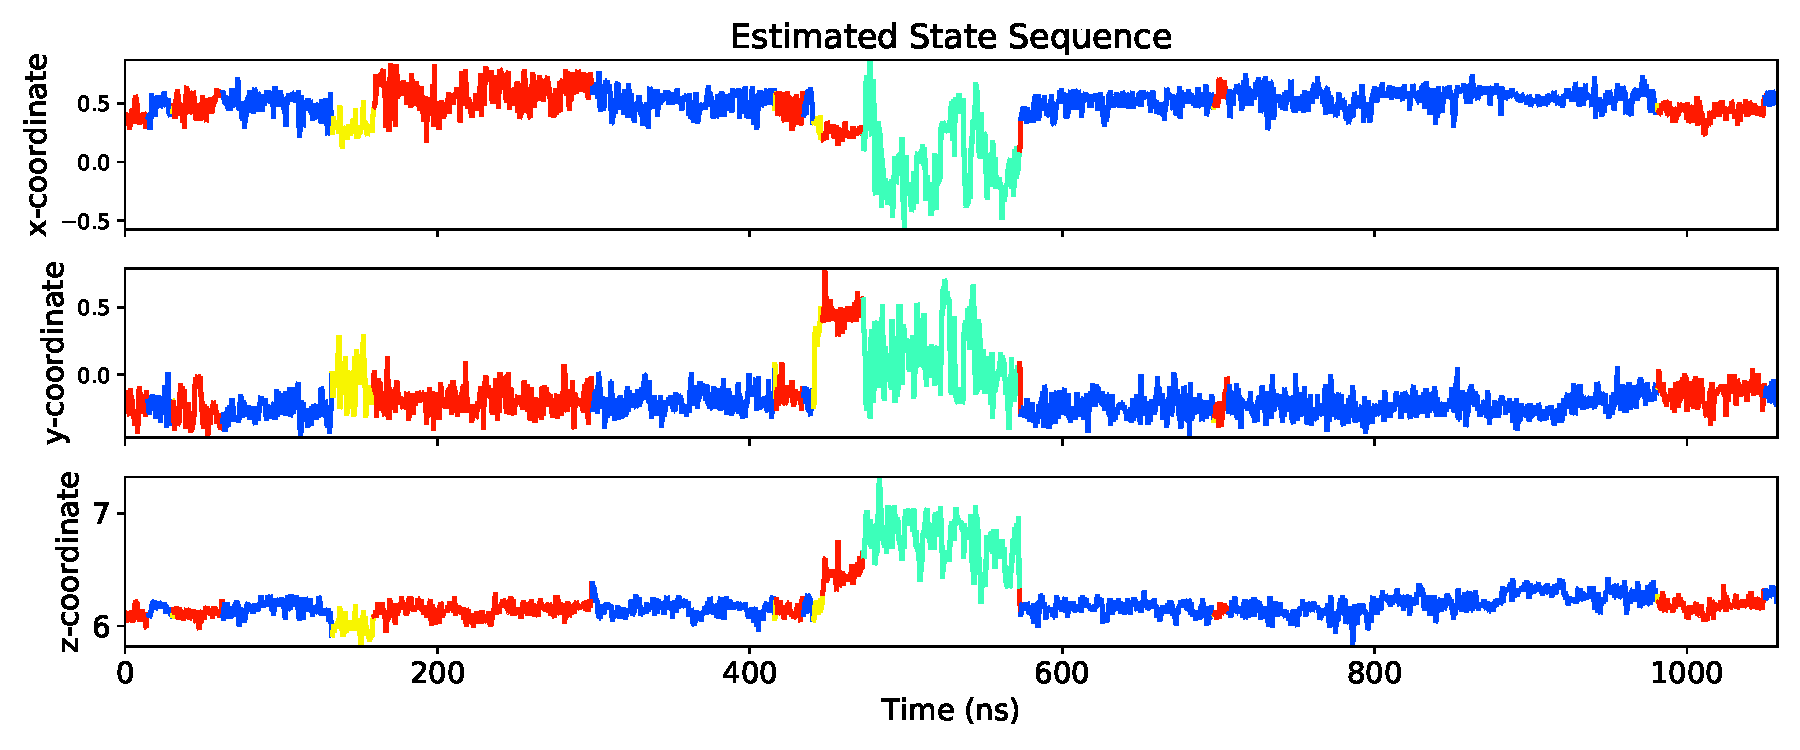
\includegraphics[width=\textwidth]{seed_ACH21_segment0.pdf}
  \caption{Found 4 Unique States}\label{fig:segment1}
  \end{subfigure}
  \begin{subfigure}{0.48\textwidth}
  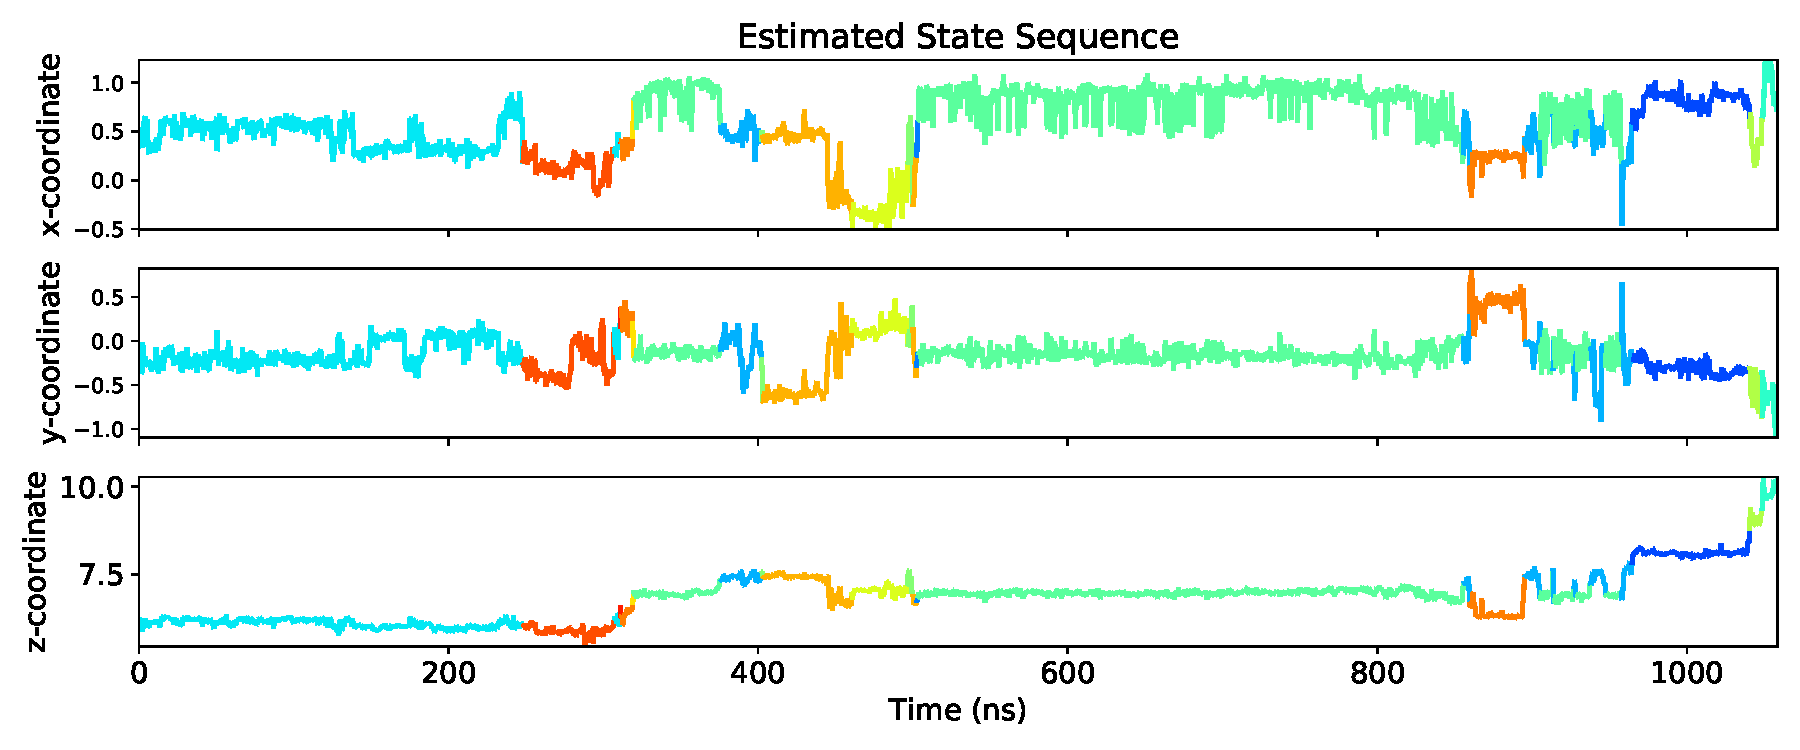
\includegraphics[width=\textwidth]{seed_ACH21_segment1.pdf}
  \caption{Found 14 Unique States}\label{fig:segment2}
  \end{subfigure}
  \begin{subfigure}{0.48\textwidth}
  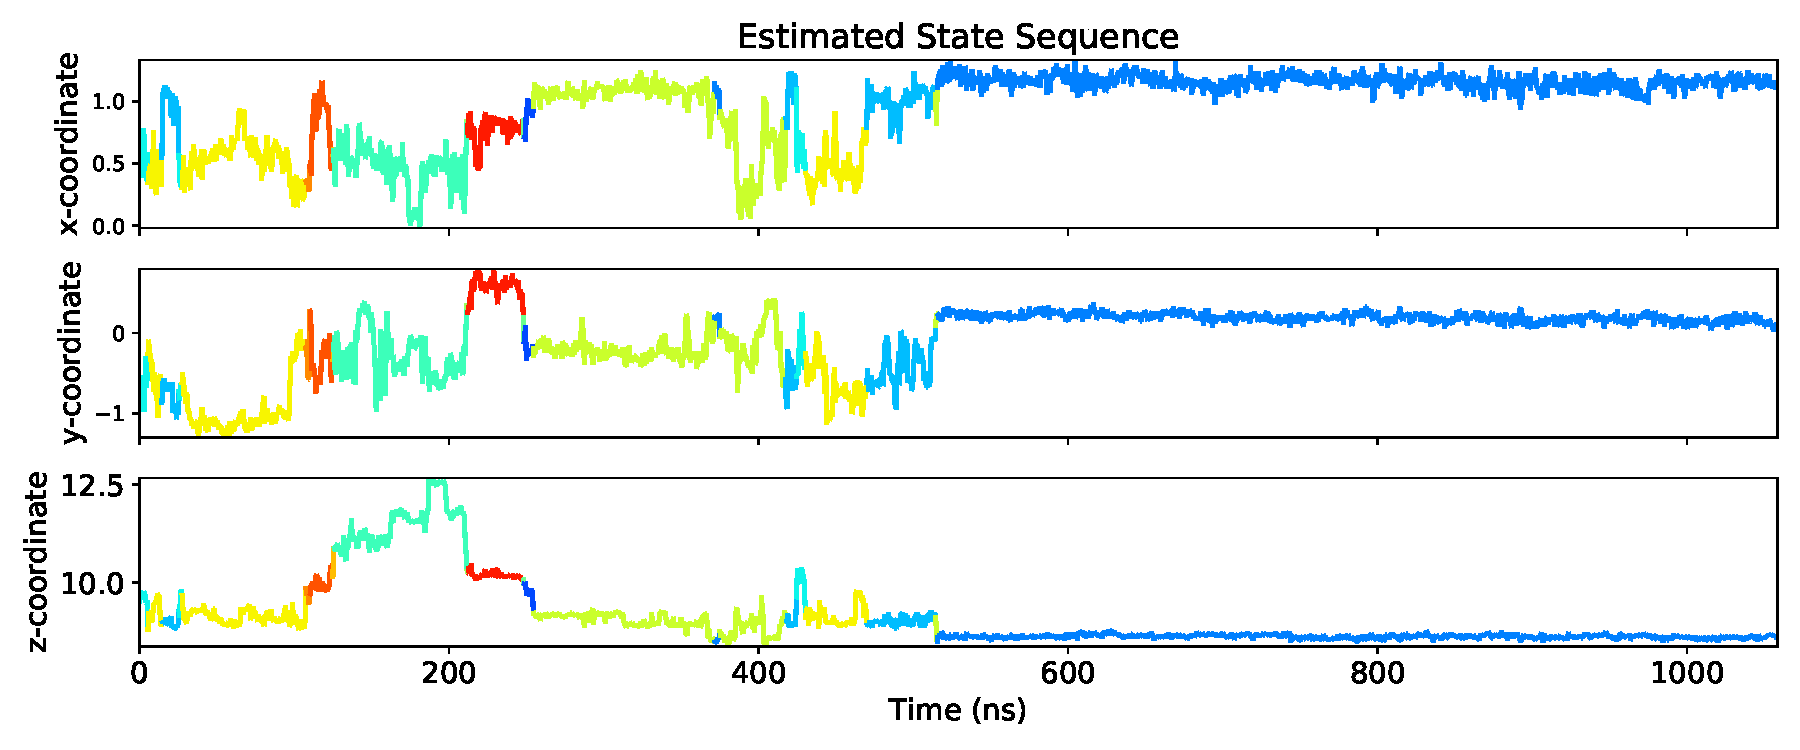
\includegraphics[width=\textwidth]{seed_ACH21_segment2.pdf}
  \caption{Found 13 Unique States}\label{fig:segment3}
  \end{subfigure}
  \begin{subfigure}{0.48\textwidth}
  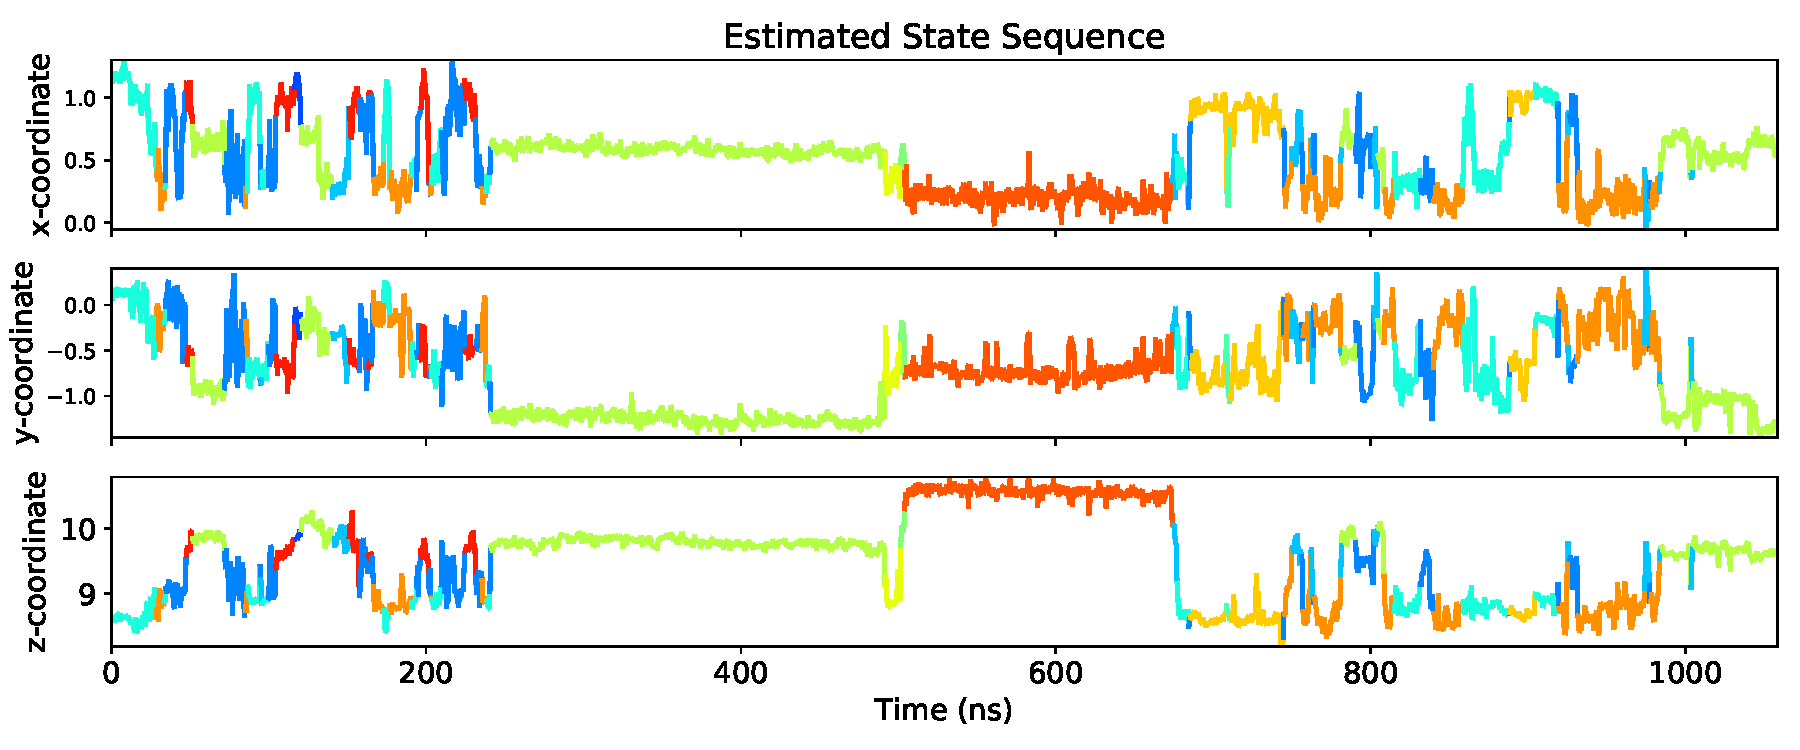
\includegraphics[width=\textwidth]{seed_ACH21_segment3.pdf}
  \caption{Found 12 Unique States}\label{fig:segment4}
  \end{subfigure}
  \begin{subfigure}{1\textwidth}
  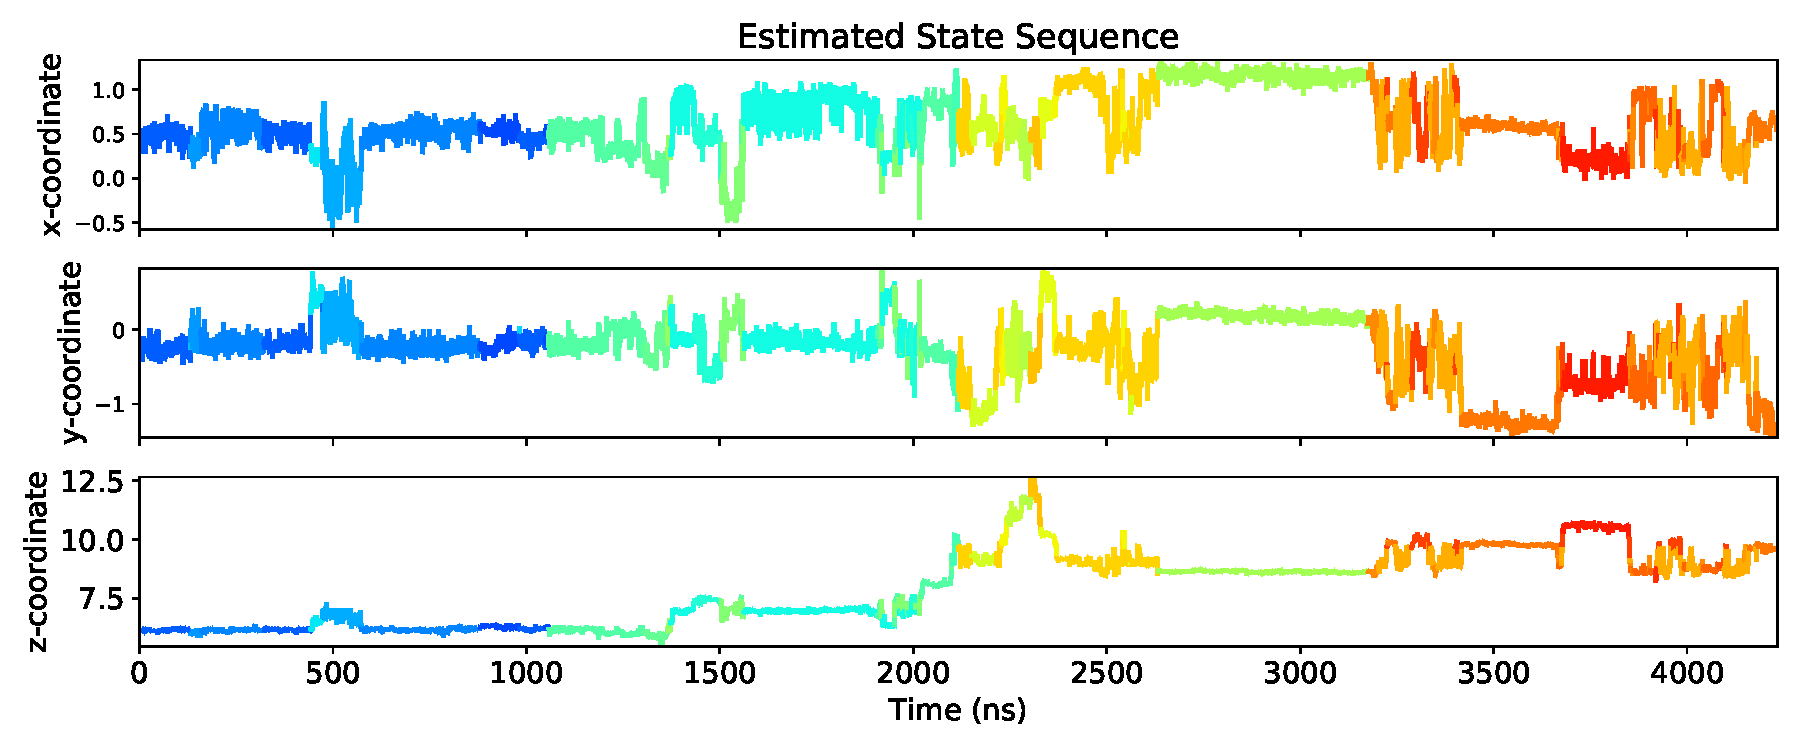
\includegraphics[width=\textwidth]{seed_ACH21_full.pdf}
  \caption{Initial state sequence seeded with states found in (a)--(d)}\label{fig:full}
  \end{subfigure}
  \caption{In (a--d), we show the state sequence resulting from 5 iterations
  of the IHMM on each of the four quarters of the center-of-mass trajectory in
  (e) after splitting it into 4 separate segments. We use the concatenation 
  of the four state sequences as the initial sequence for the IHMM run on the 
  fully trajectory in (e).
  }\label{fig:seed_sequence}
  \end{figure}
  
  \section{Clustering}\label{section:clustering}
  
  \subsection{Agglomerative Clustering Versus Gaussian Mixture Models}\label{section:agglomerative}
  
  % BJC: will show Gaussian mixture model which has a cluster engulfing another cluster, so
  % it's tails are on both sides of the center cluster.
  
  \begin{figure}[h]
  \centering
  \begin{subfigure}{0.95\textwidth}
  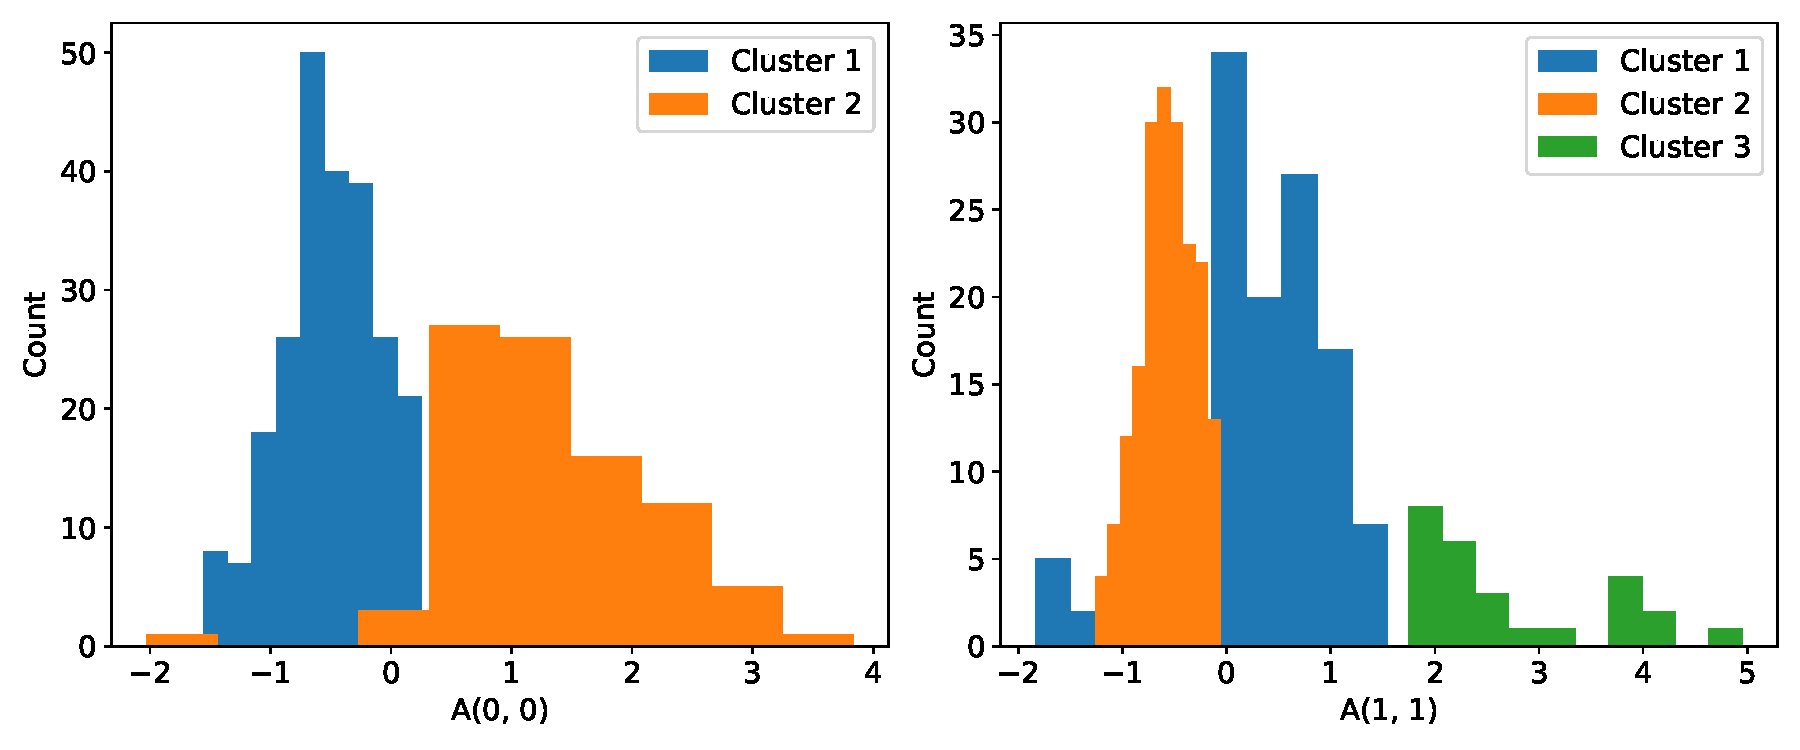
\includegraphics[width=\textwidth]{bayesian_A.pdf}
  \caption{Bayesian Gaussian mixture model}\label{fig:bayesian_A}
  \end{subfigure}
  \begin{subfigure}{0.95\textwidth}
  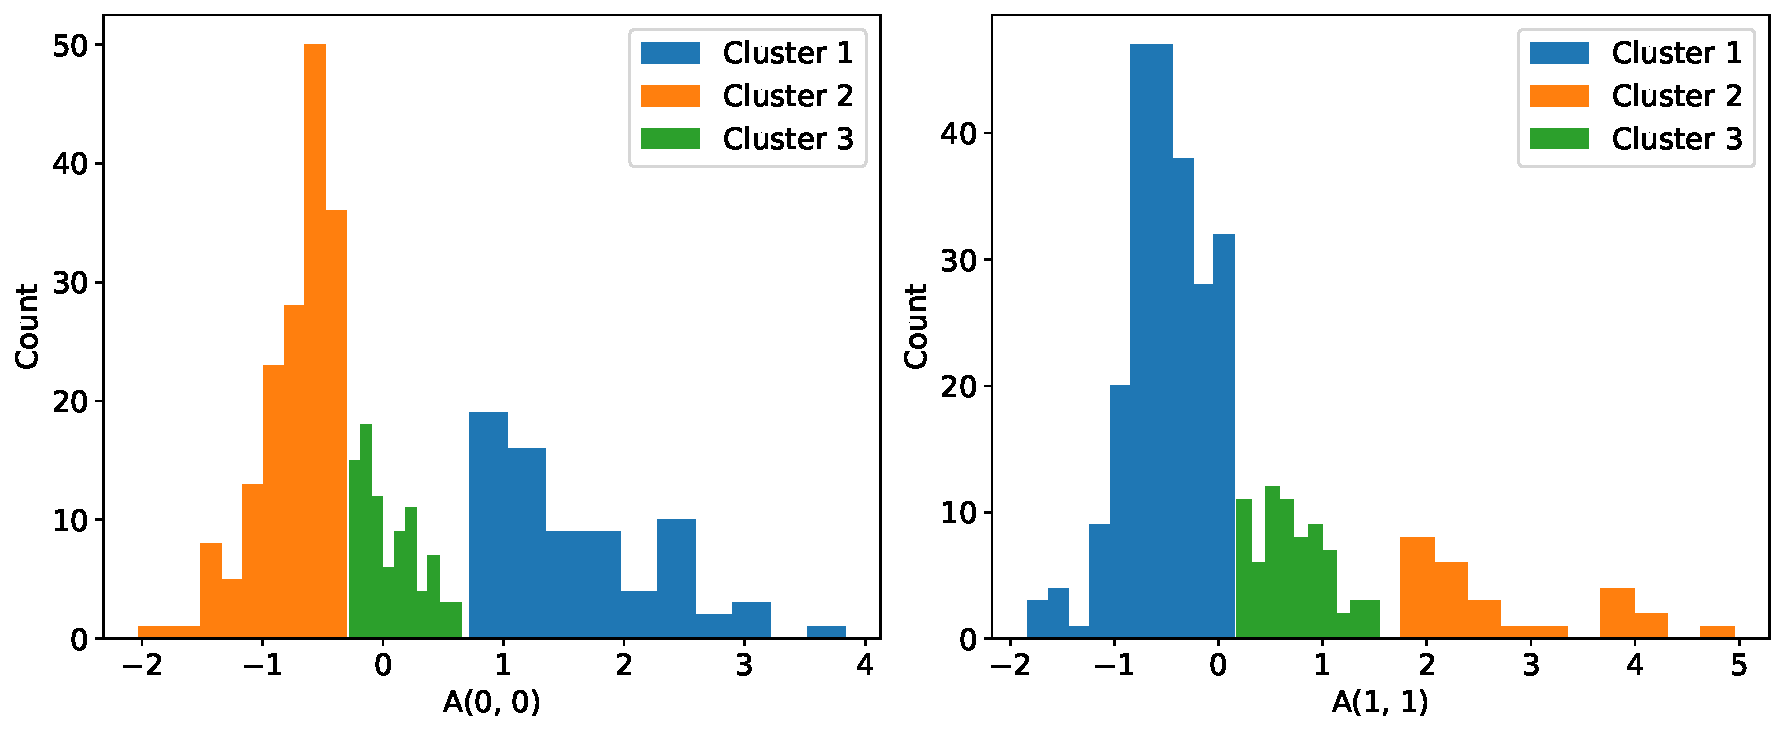
\includegraphics[width=\textwidth]{agglomerative_A.pdf}
  \caption{Agglomerative Clustering}\label{fig:agglomerative_A}
  \end{subfigure}
  \caption{To reduce the state space, we prefer agglomerative clustering over Bayesian
  Gaussian mixture modeling. In the plots above we show the results of clustering the
  diagonal entries of the autoregressive coefficient matrices, $A$, of methanol. (a) 
  Bayesian Gaussian mixture models tend to delocalize the clusters in parameter space
  since the Gaussians can overlap. Agglomerative clustering prevents overlap of 
  clusters and ensures that all states within each cluster have similar parameters.
  }\label{fig:clustering_choice}
  \end{figure}
  
  \newpage
  
%  \subsection{Clustering on the self-transition probabilities}\label{section:selfT_cluster}
%  
%  To cluster on $T_{ii}$, we first cast it in terms of the expected dwell times. The expected 
%  value of the number of sequential self-transitions is simply $\frac{1}{1 - T_{ii}}$. This 
%  relationship correctly implies that dwell times approach infinity as $T_{ii}$ approaches 1. 
%  There we found the most success with agglomerative clustering by linearizing this 
%  relationship and clustering on $-log(1 - T_{ii})$.
  
  \subsection{Choosing Linkage Criteria and the Number of Clusters}\label{section:nclusters}
  
  In this section, we determine the optimal linkage criteria and number of clusters
  for studying methanol's parameters. We applied the same workflow to make analogous
  decisions for ethylene glycol, urea and acetic acid. In all cases, we found that
  the `ward' linkage criteria resulted in the most useful clustering. We chose to 
  use x number of clusters for each solute, the minimum number of clusters, by our
  analysis, needed to adequately distinguish state dynamics. 
  
  In order to cluster the parameter sets, we need to determine the linkage criteria 
  that will be used to measure the distance between clusters as well as an appropriate
  total number of clusters. In Figure~\ref{fig:linkages}, we show the result of clustering
  with each type of linkage criteria available with the 
  \texttt{sklearn.cluster.AgglomerativeClustering} class of the \texttt{scikit-learn} 
  python package. It is clear that both the `average' and `single' linkage criteria 
  do not sufficiently cluster the data. The `ward' criteria appears to result in the 
  highest number of large population clusters.
  
  \begin{figure}
  \centering
  \begin{subfigure}{0.24\textwidth}
  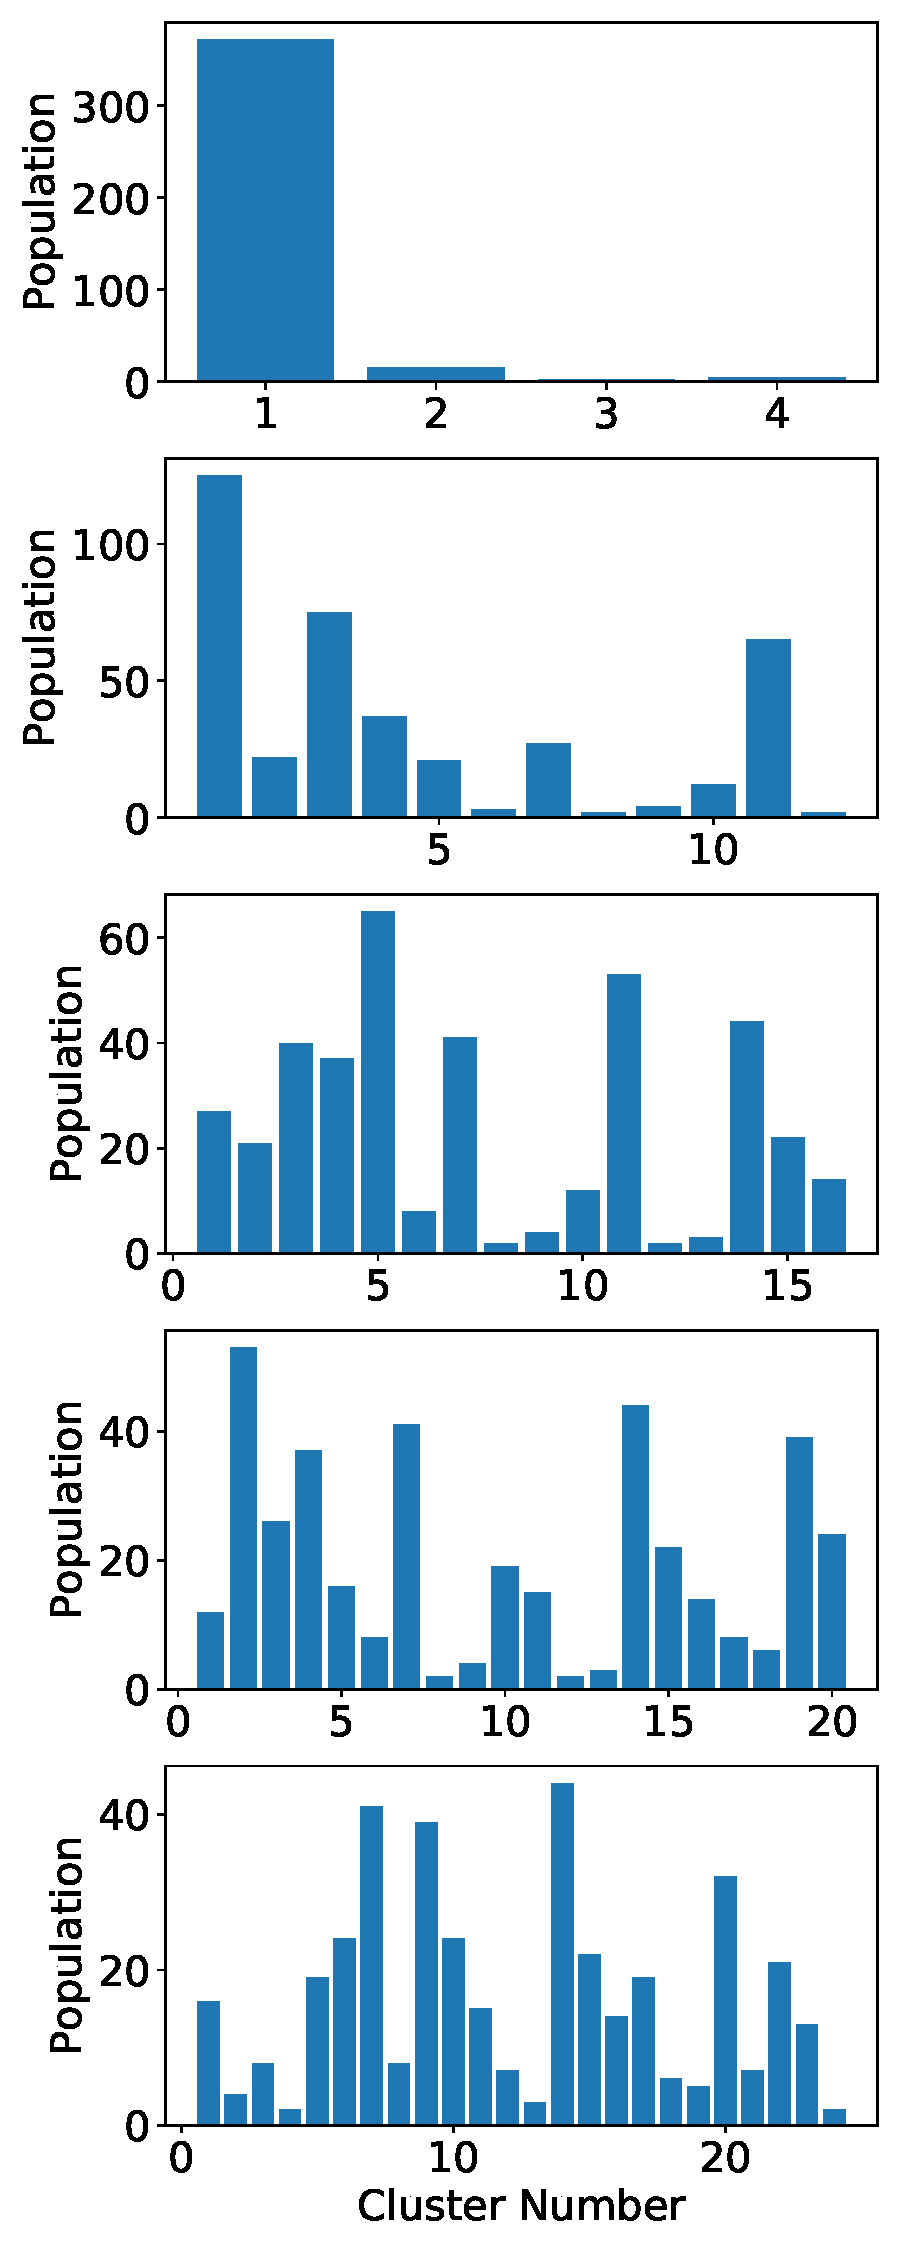
\includegraphics[width=\textwidth]{nclusters_ward.pdf}
  \caption{`ward'}\label{fig:nclusters_ward}
  \end{subfigure}
  \begin{subfigure}{0.24\textwidth}
  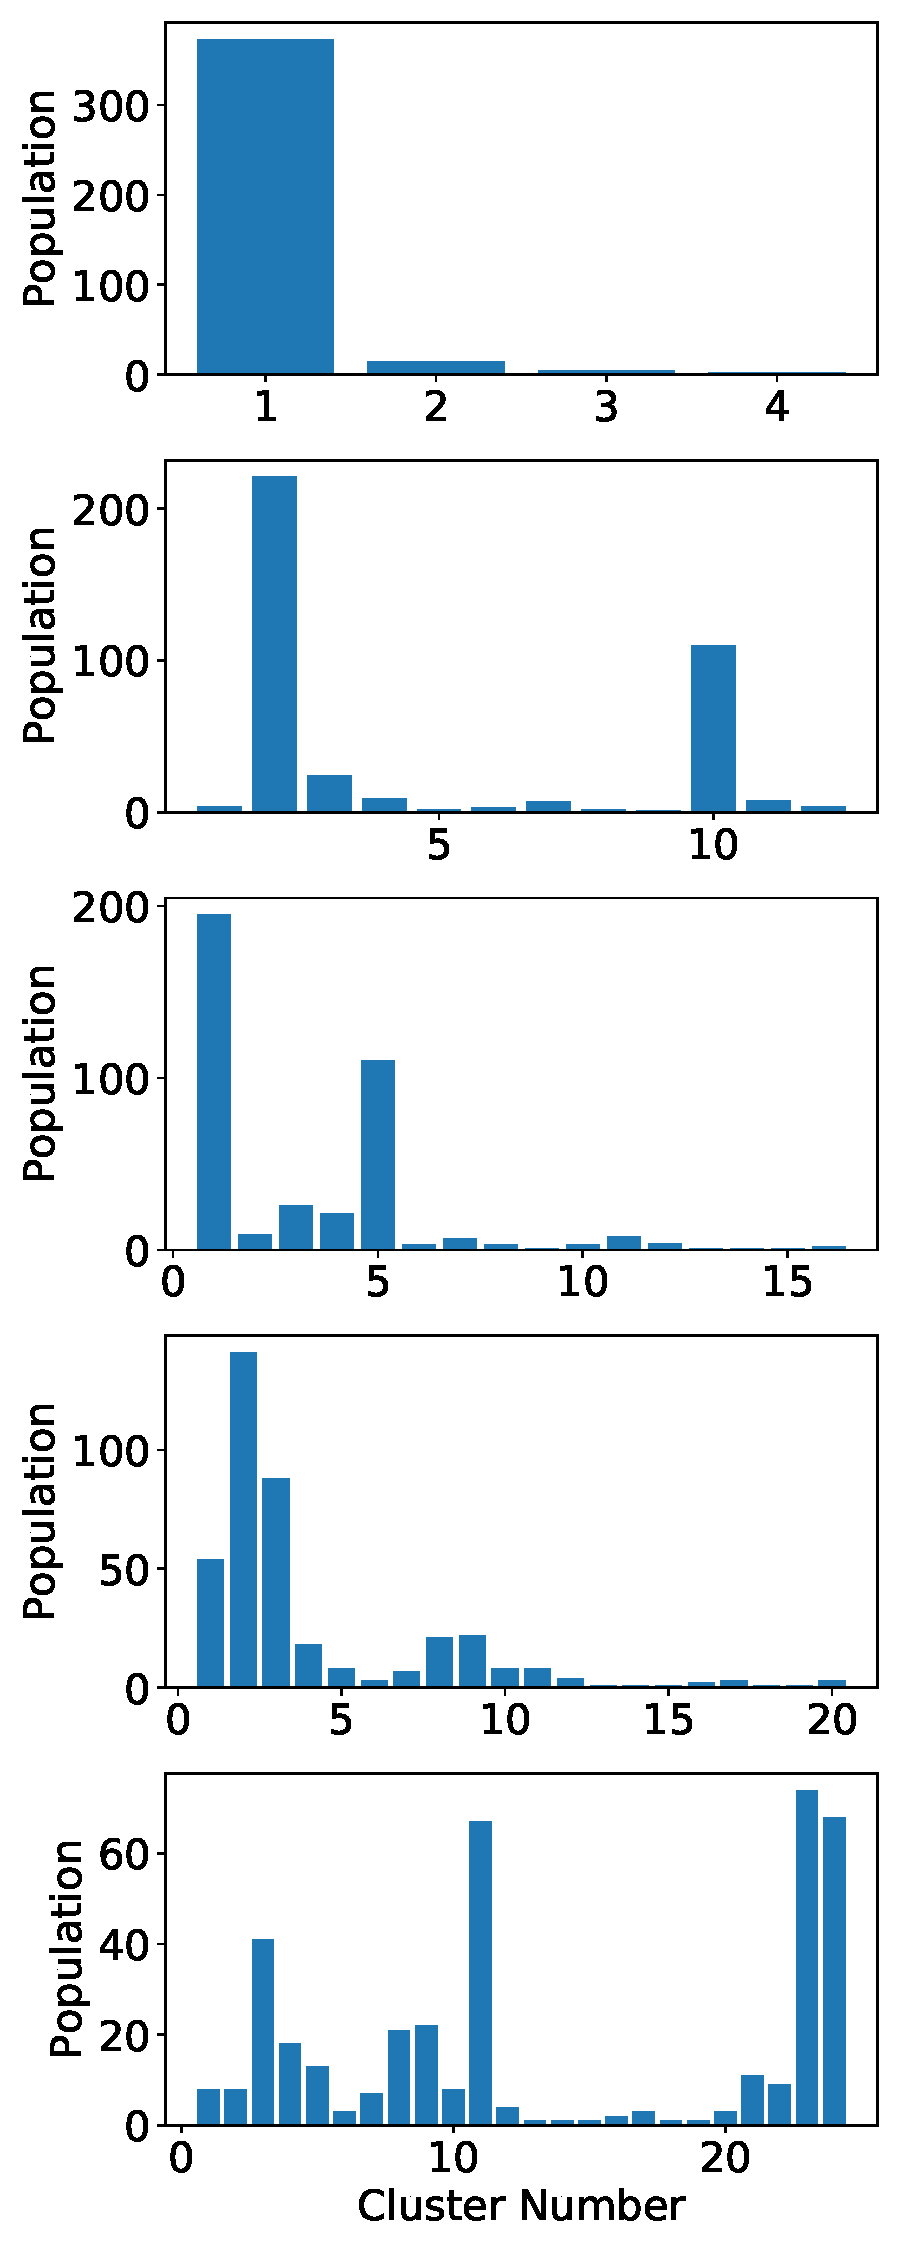
\includegraphics[width=\textwidth]{nclusters_complete.pdf}
  \caption{`complete'}\label{fig:silhouette_URE}
  \end{subfigure}
  \begin{subfigure}{0.24\textwidth}
  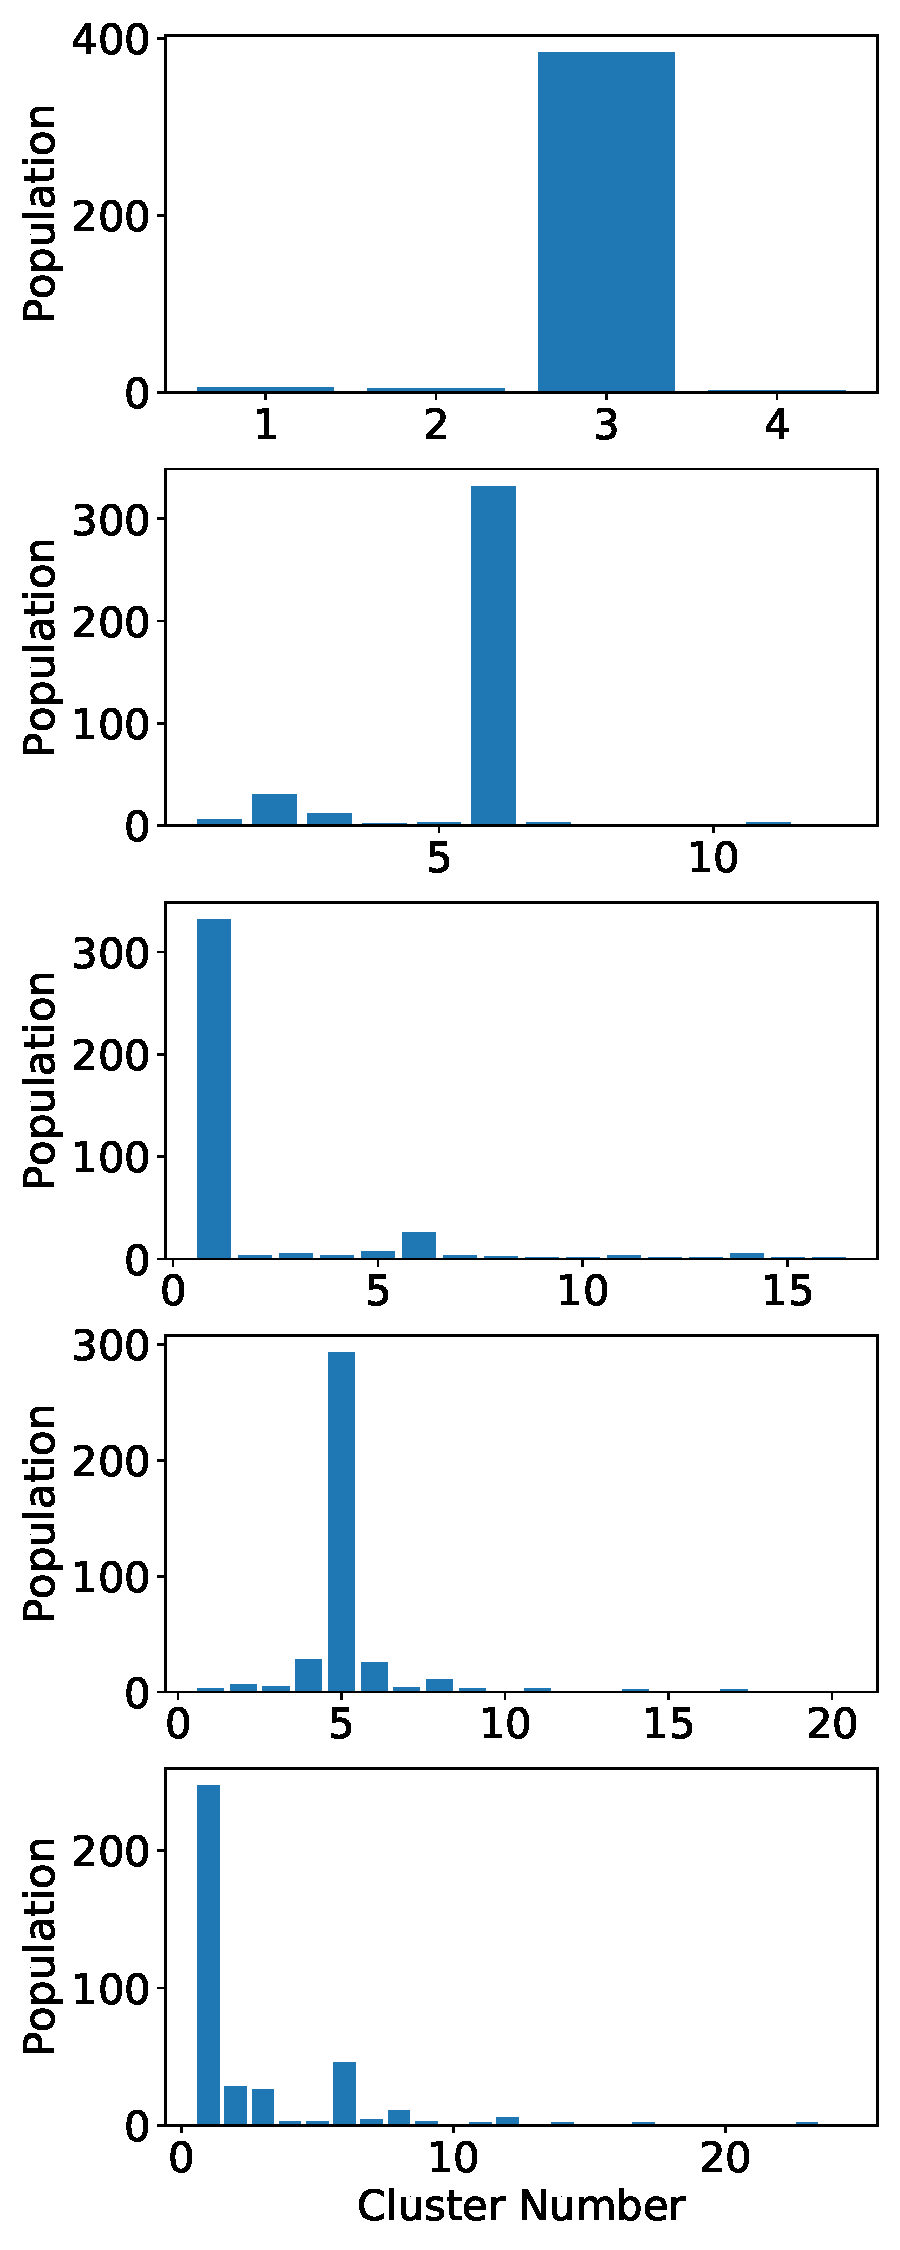
\includegraphics[width=\textwidth]{nclusters_average.pdf}
  \caption{`average'}\label{fig:nclusters_average}
  \end{subfigure}
  \begin{subfigure}{0.24\textwidth}
  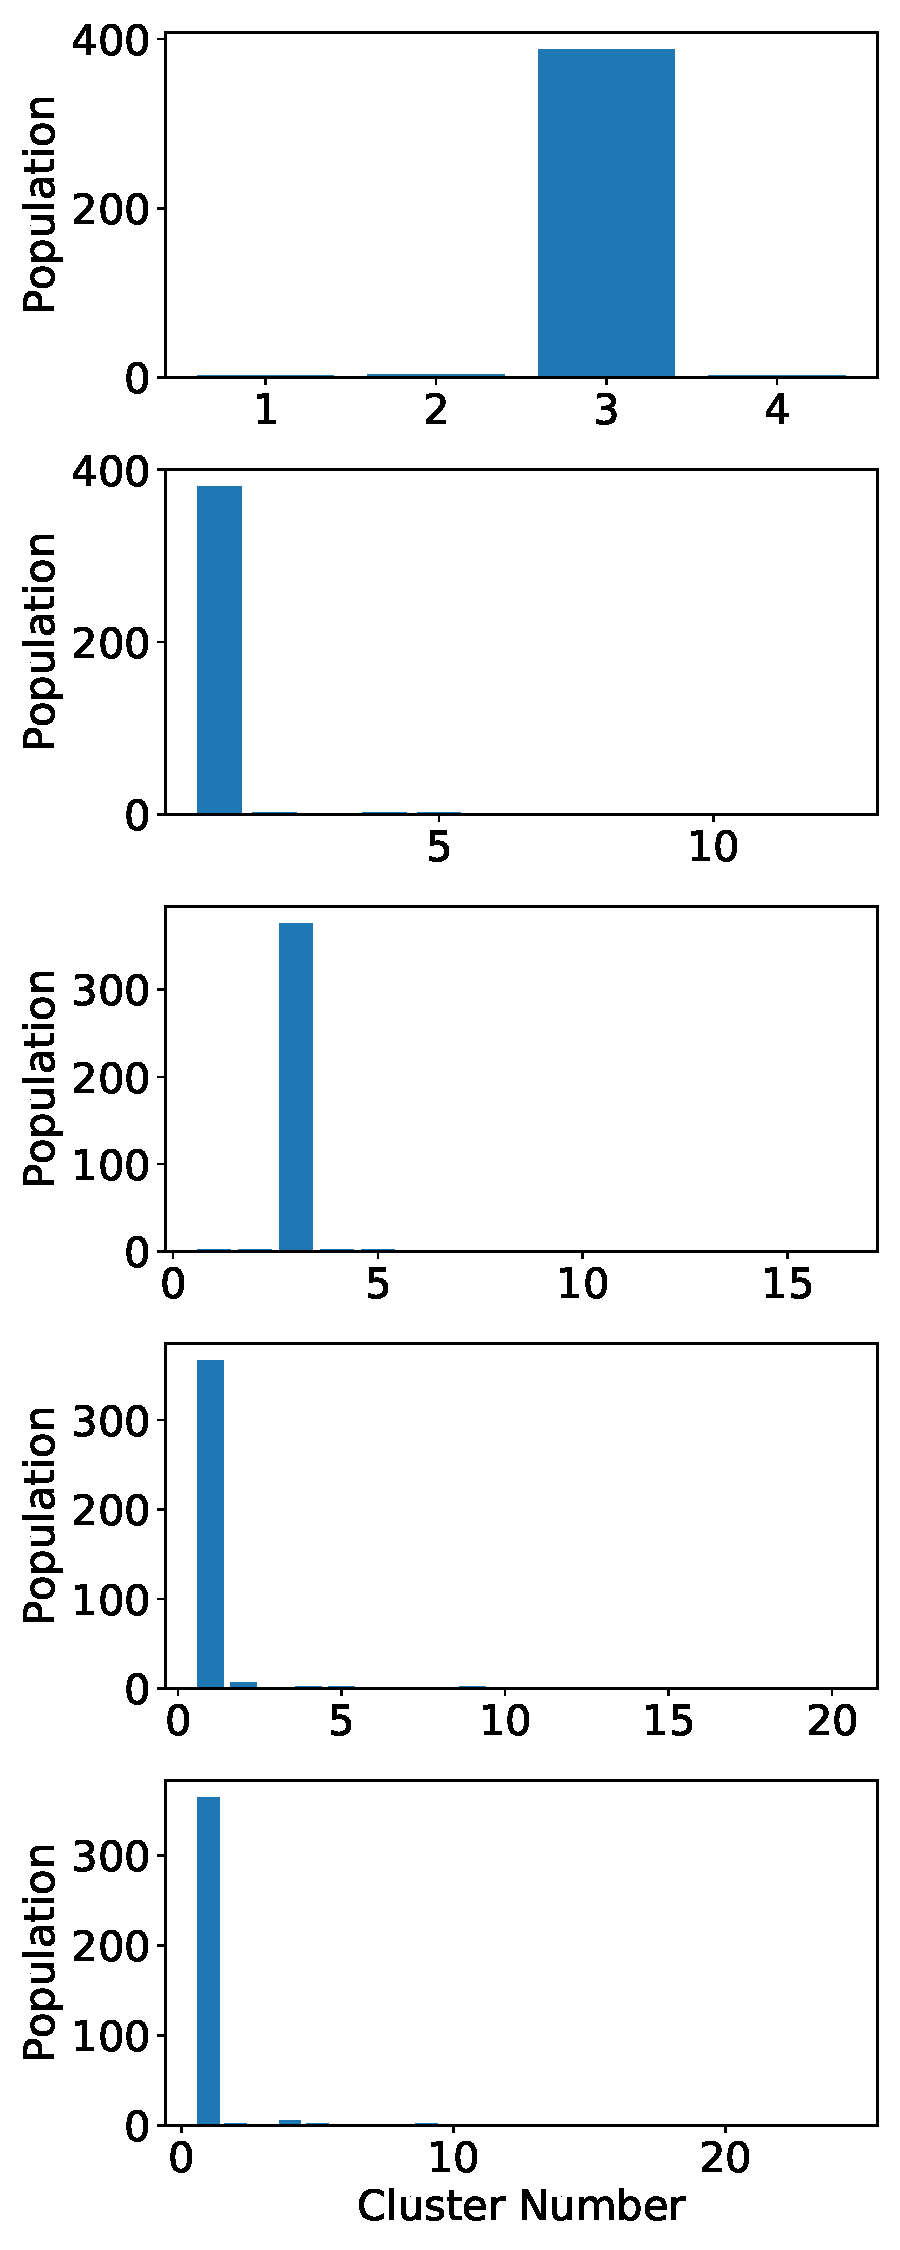
\includegraphics[width=\textwidth]{nclusters_single.pdf}
  \caption{`single'}\label{fig:nclusters_single}
  \end{subfigure}
  \caption{In each column we tested a different linkage criteria for clustering
  of the methanol parameters. In each row, we varied the number of total clusters. 
  Both `ward' and `complete' linkage appear to induce clustering
  while the `average' and `single' criteria tend to concentrate parameters in
  only a fraction of the available clusters.}\label{fig:linkages}
  \end{figure}
  
  We can help to further narrow our decision of linkage criteria by analyzing 
  the parameters of the clusters which it produces. In particular, we should 
  look for well-distinguished clusters on the radial means so that it will be
  easier to connect solute behavior to the membrane pore structure. One way to
  concisely visualize the radial clusters is by their spread. An optimal number
  of clusters should have the same spread in radial means as the unclustered
  data. In Figure~\ref{fig:rspread}, we show that `ward' linkage results in 
  the highest spread in the radials means of the clusters across a range of
  4--30 total clusters. For a low to intermediate number of clusters, the 
  spread of `ward' clusters is significantly larger than of the other linkage
  methods. Therefore, we have chosen to use `ward' clustering.
  
  We use the Silhouette score in order to aid us in choosing the total number of
  clusters. In Figure~\ref{fig:silhouette_MET}, we plot the Silhouette score as
  a function of the total number of clusters using the `ward' linkage criteria. 
  A Silhouette score of 1 indicates the best clustering possible, values near
  0 indicate overlapping clusters, and negative values indicate samples belong to
  the wrong clusters. For the methanol parameters, the Silhouette score drops off
  quickly with number of clusters before plateauing around 7 total clusters. 
  However, given the low spread in $\mu_r$, it is not clear that using 7 or less 
  clusters will give useful clustering results.
  
  \begin{figure}
  \centering
  \begin{subfigure}{0.53\textwidth}
  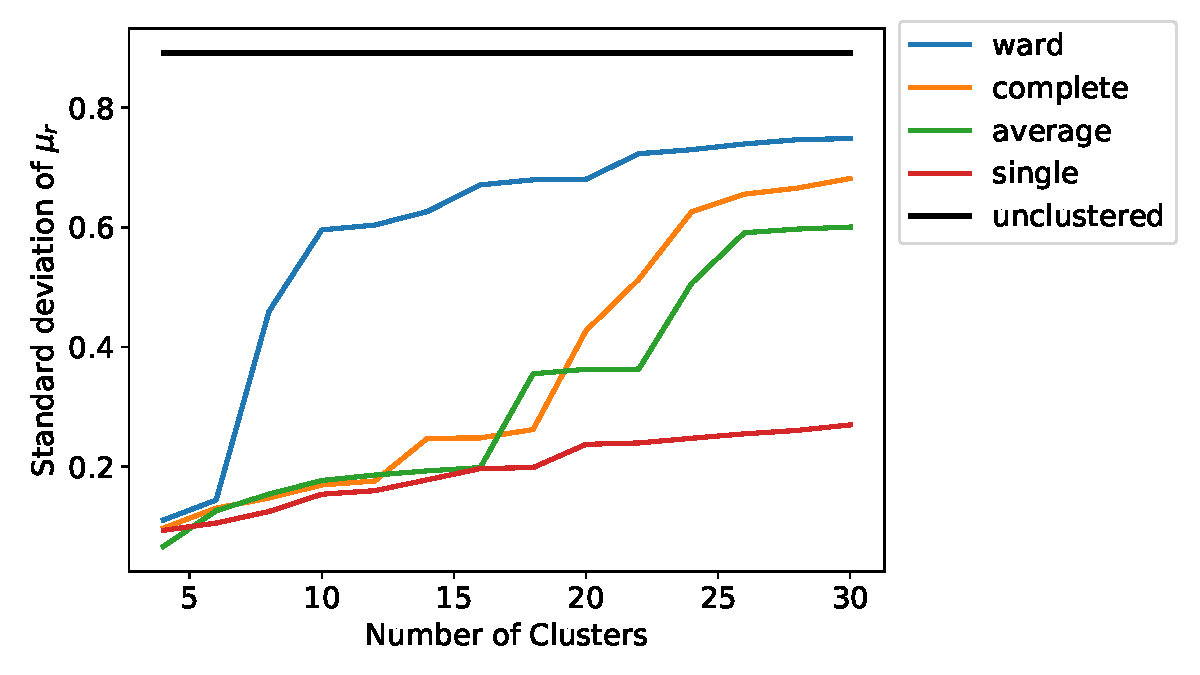
\includegraphics[width=\textwidth]{rspread_nclusters.pdf}
  \caption{}\label{fig:rspread}
  \end{subfigure}
  \begin{subfigure}{0.45\textwidth}
  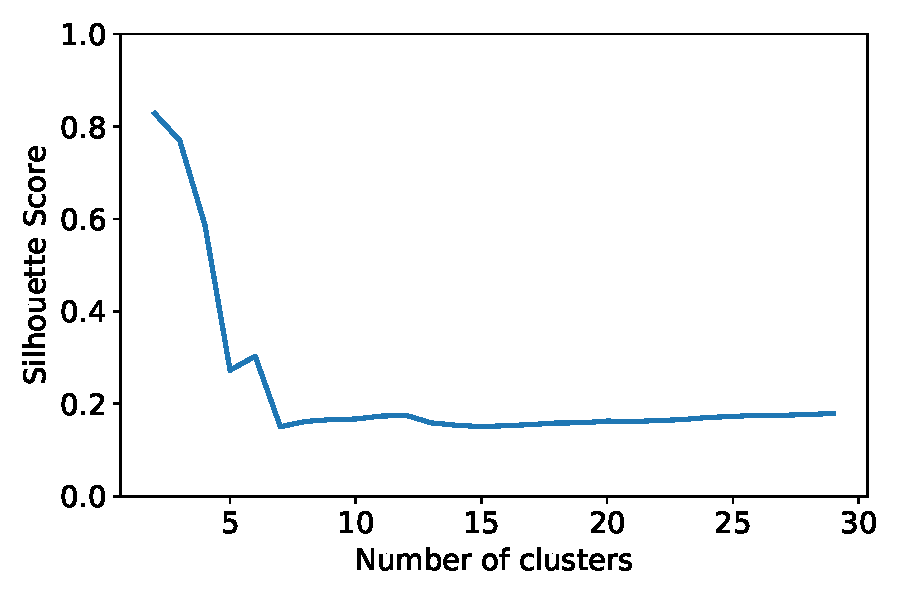
\includegraphics[width=\textwidth]{silhouette_MET.pdf}
  \caption{}\label{fig:silhouette_MET}
  \end{subfigure}
  \caption{(a) The `ward' linkage criteria maintains the highest standard 
  deviation in radial means, $\mu_r$, of the clusters for a given total 
  number of clusters as compared to other linkage criteria. (b) The 
  Silhouette score, used to evaluate the quality of clustering with the 
  `ward' distance criteria drops precipitously as a function of the chosen
  total number of clusters before plateauing.}\label{fig:idk}
  \end{figure}
  
  We incorporate qualitative feedback into the decision on the number of 
  clusters. Despite its high Silhouette score, Figure~\ref{fig:4cluster_state_sequence}
  illustrates that using 4 clusters clearly does not distinguish dynamical 
  modes. We do not see visually acceptable clustering on the example trajectory
  until we use at least twenty total clusters (Figure~\ref{fig:20cluster_state_sequence}).
  
  \begin{figure}
  \begin{subfigure}{0.9\textwidth}
  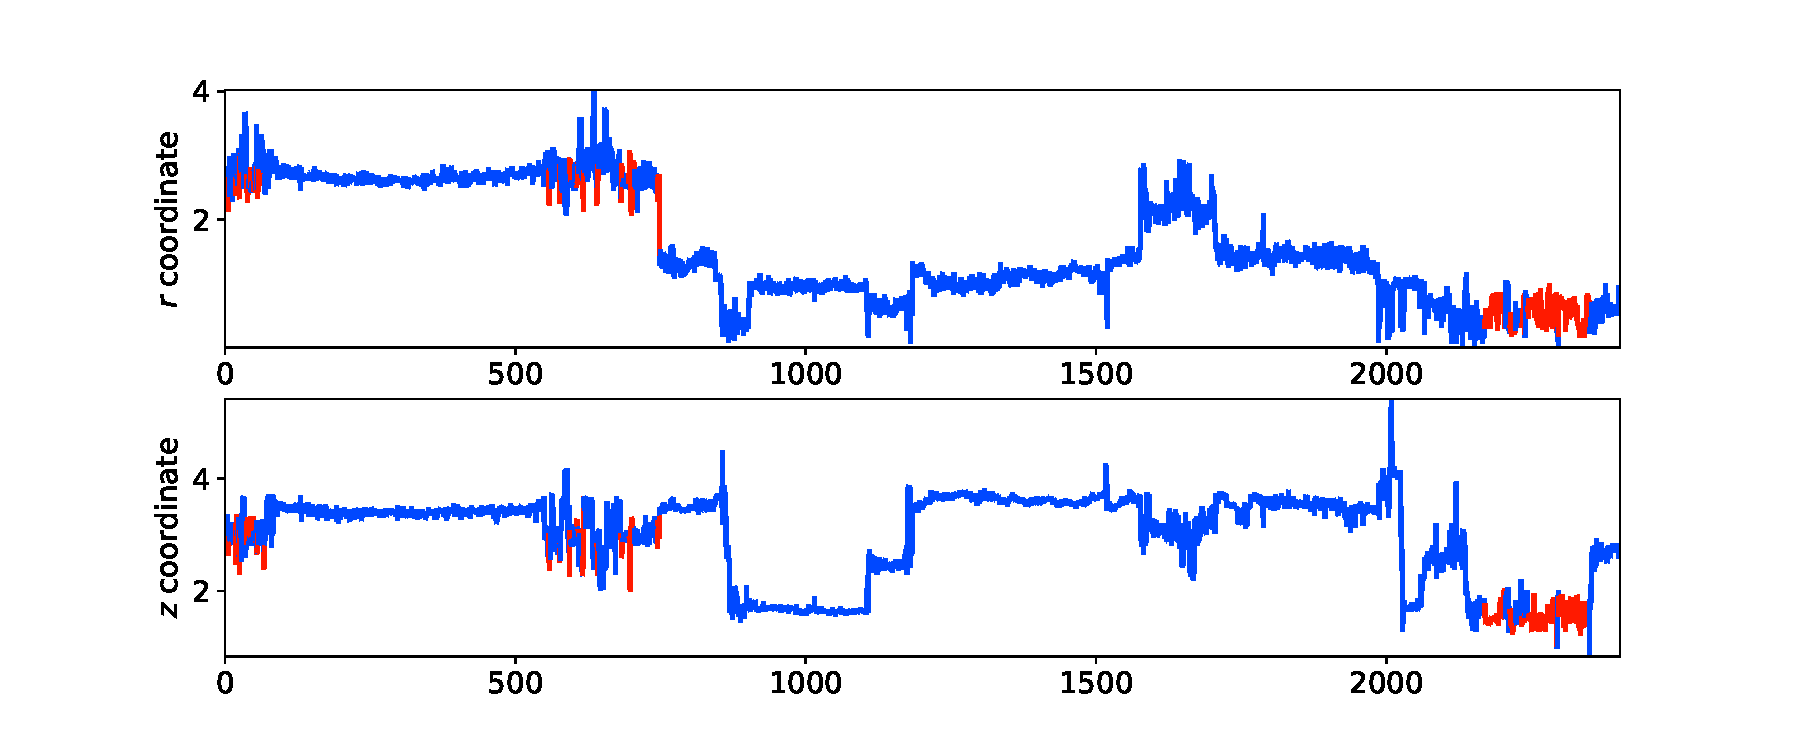
\includegraphics[width=1\textwidth]{clustered_traj_MET_ward_4.pdf}
  \caption{4 total clusters}\label{fig:4cluster_state_sequence}
  \end{subfigure}
  \begin{subfigure}{0.9\textwidth}
  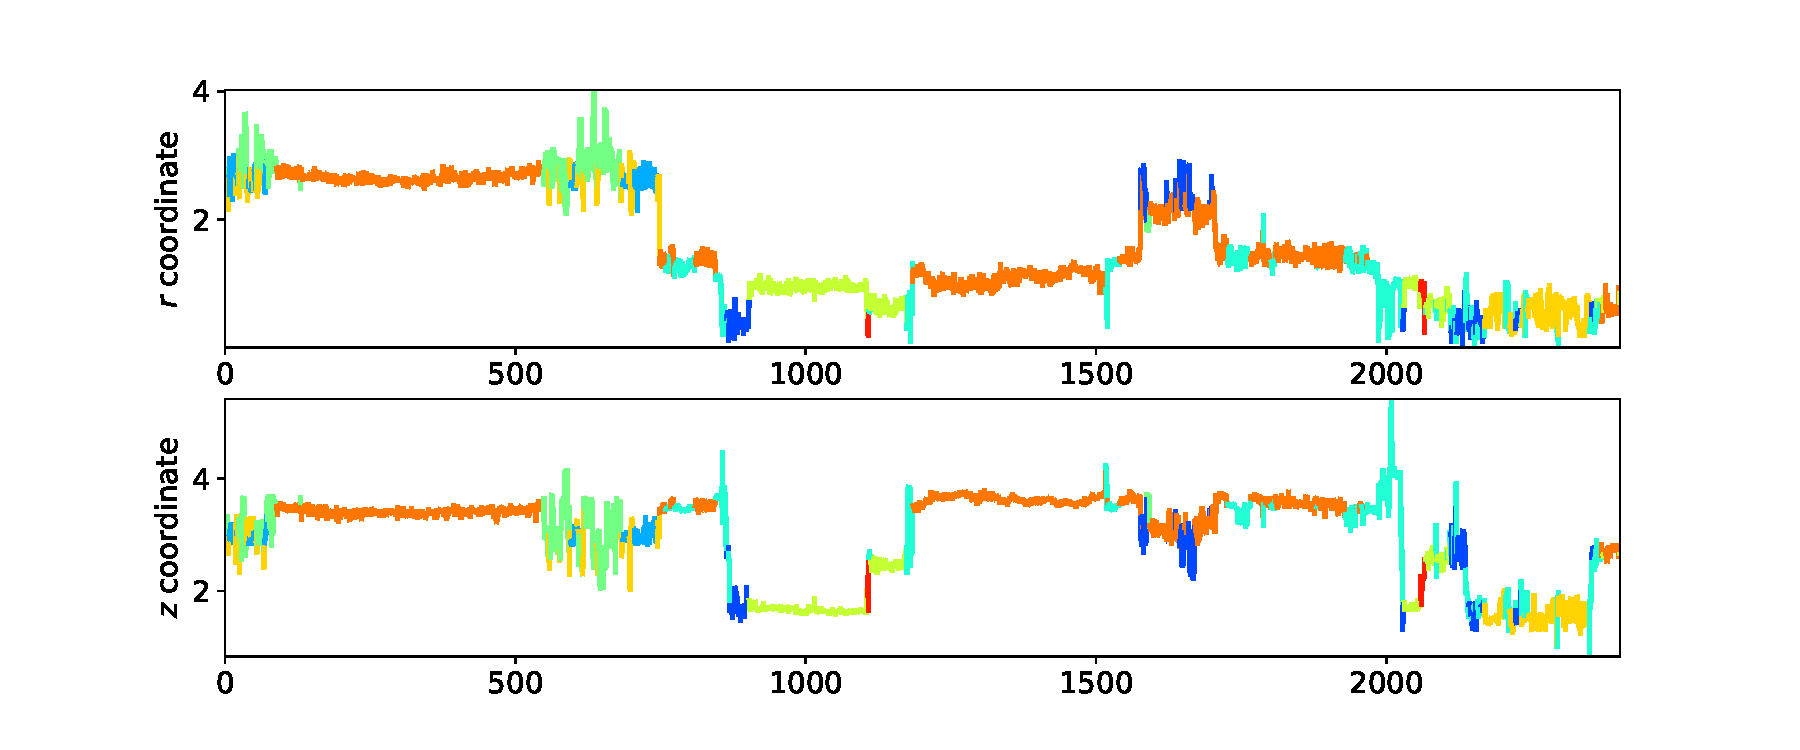
\includegraphics[width=1\textwidth]{clustered_traj_MET_ward_12.pdf}
  \caption{12 total clusters}\label{fig:12cluster_state_sequence}
  \end{subfigure}
  \begin{subfigure}{0.9\textwidth}
  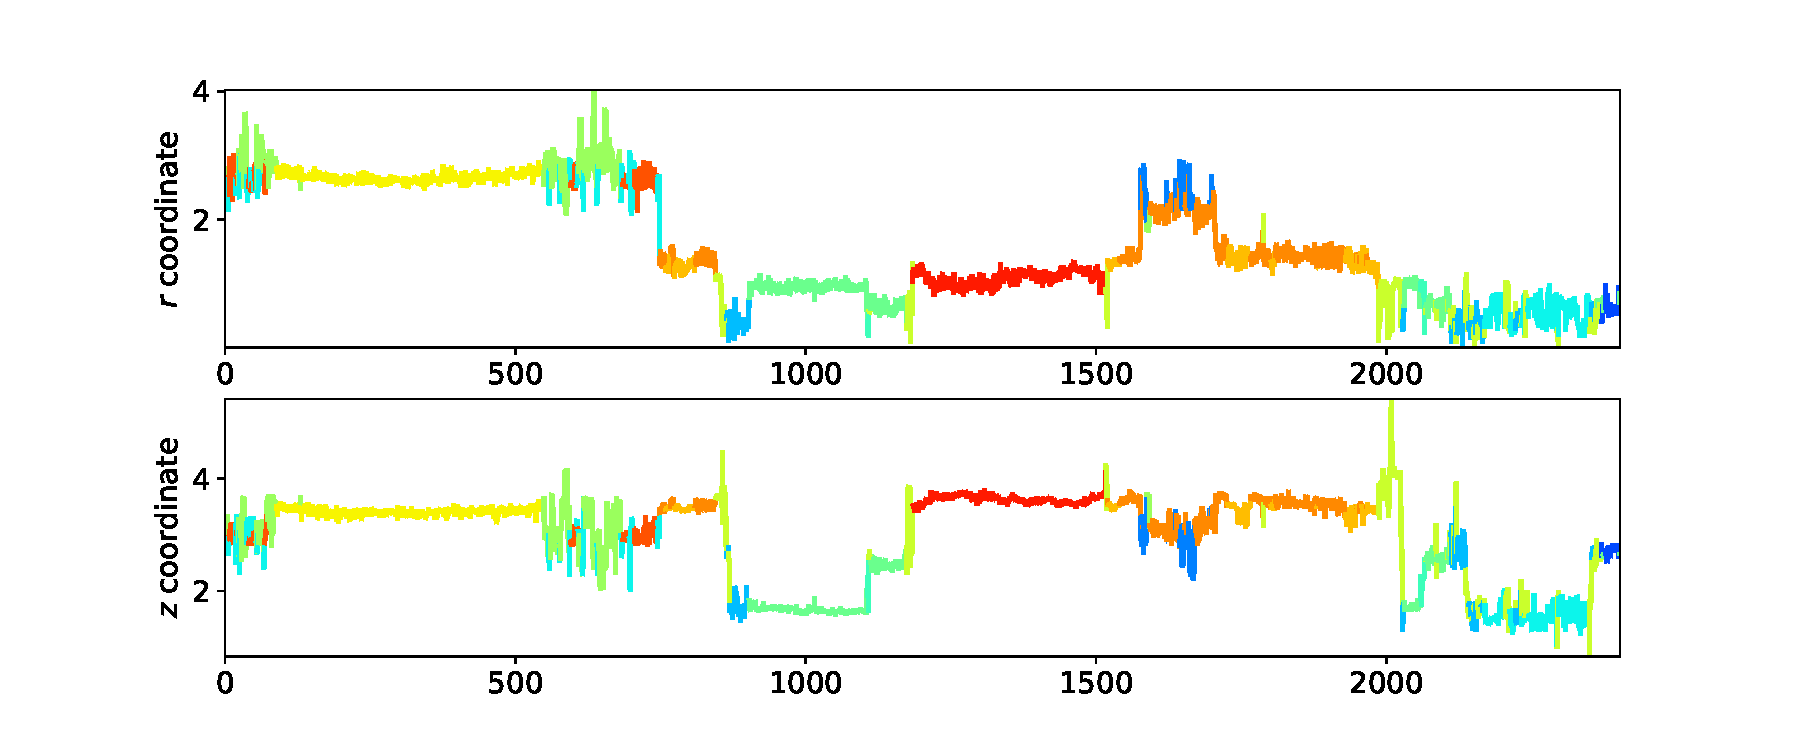
\includegraphics[width=1\textwidth]{clustered_traj_MET_ward_20.pdf}
  \caption{20 total clusters}\label{fig:20cluster_state_sequence}
  \end{subfigure}
  \caption{Although the Silhouette score for four total clusters is high, we do
  not see adequate distinction between clusters until we group the parameters
  from the 24 trajectories into 20 total clusters. When we use 12 total clusters,
  the distinction appears acceptable except that the segment from ~50--550 ns
  and from 1200--1500 ns (both colored orange) are clustered together. The radial
  means of these two segments correspond to two very different morphological
  regions of the membrane.}\label{fig:clustered_state_sequences}
  \end{figure}
  
  \begin{figure}
  \centering
  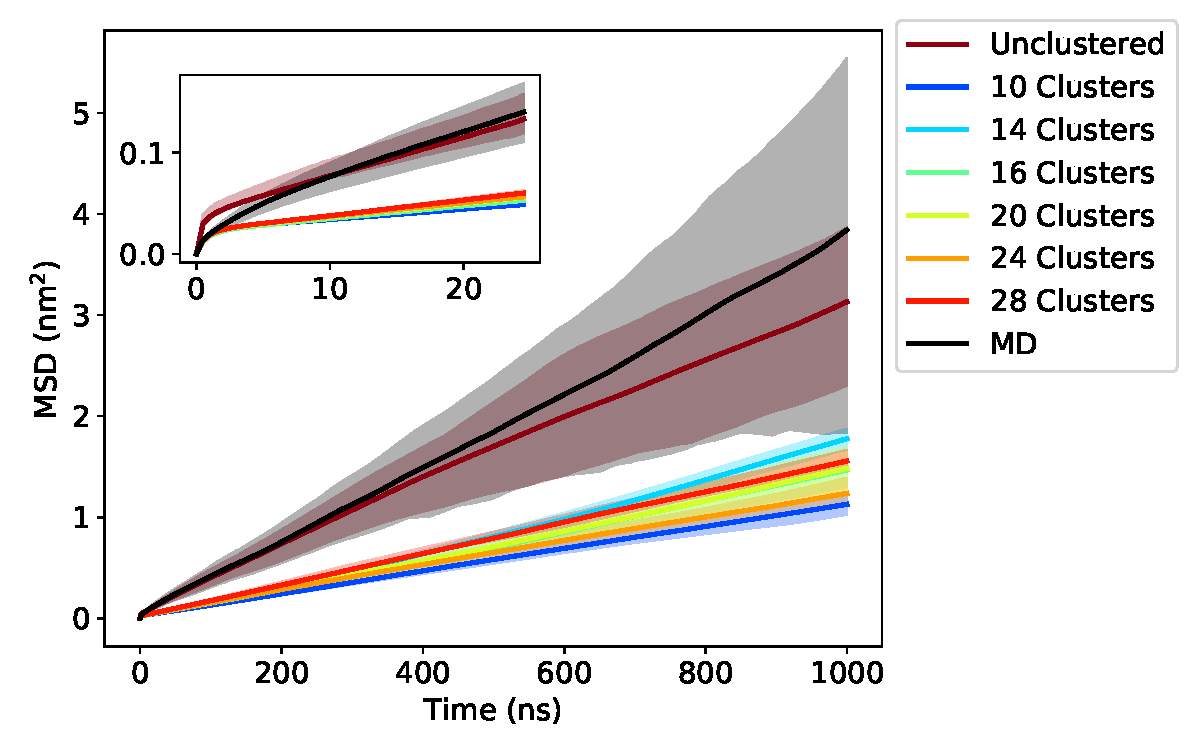
\includegraphics[width=0.7\textwidth]{nclusters_msd_MET_ward.pdf}
  \caption{The total MSD predicted by stochastic realizations of the clustered
  model is relatively insensitive to the total number of clusters. All
  predictions are less than the predictions of MD and the unclustered trajectories.
  This behavior is expected due to underestimation of the short dwell time 
  densities as described in Section~\ref{M-section:unclustered_MSD_prediction}
  of the main text.}\label{fig:MET_nclusters} 
  \end{figure}
  
  This clustering analysis will be finished after some mechanistic studies. It is
  clear that we will need some understanding of mechanisms in order to 
  arrive at a cluster recommendation.
  
%  \begin{figure}[h]
%  \centering
%  \begin{subfigure}{0.475\textwidth}
%  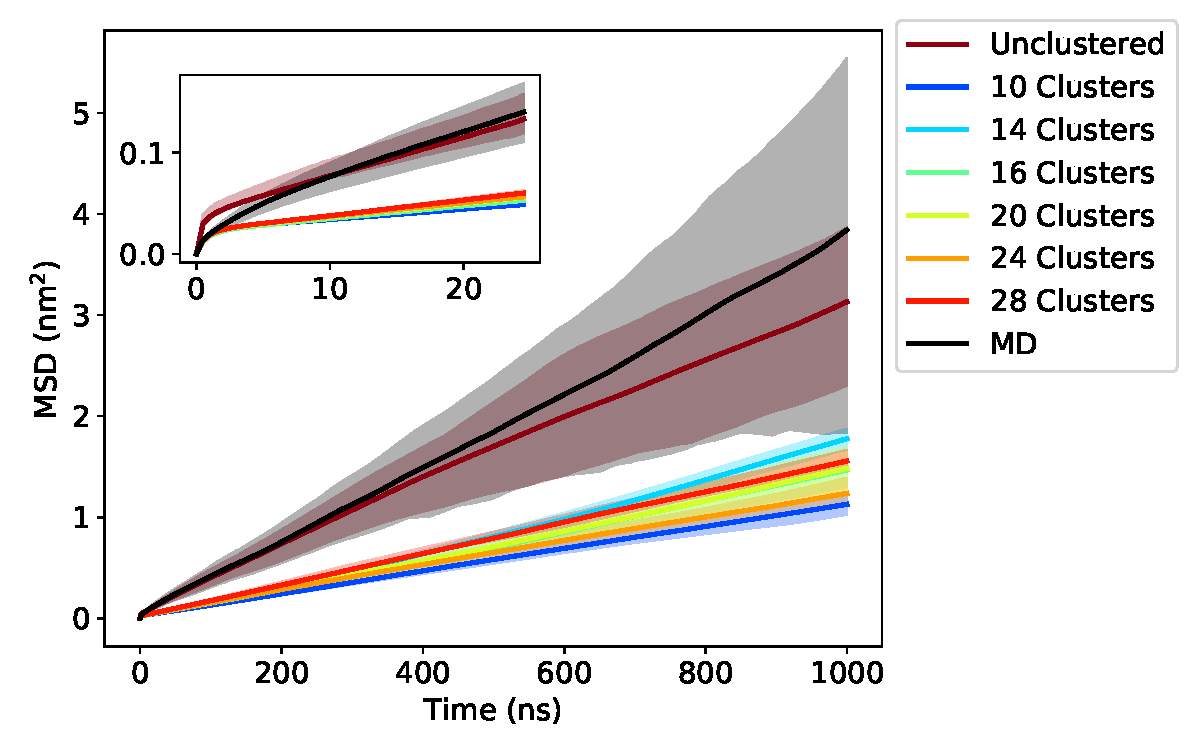
\includegraphics[width=\textwidth]{nclusters_msd_MET_ward.pdf}
%  \caption{ward}\label{fig:nclusters_msd_MET_ward}
%  \end{subfigure}
%  \begin{subfigure}{0.475\textwidth}
%  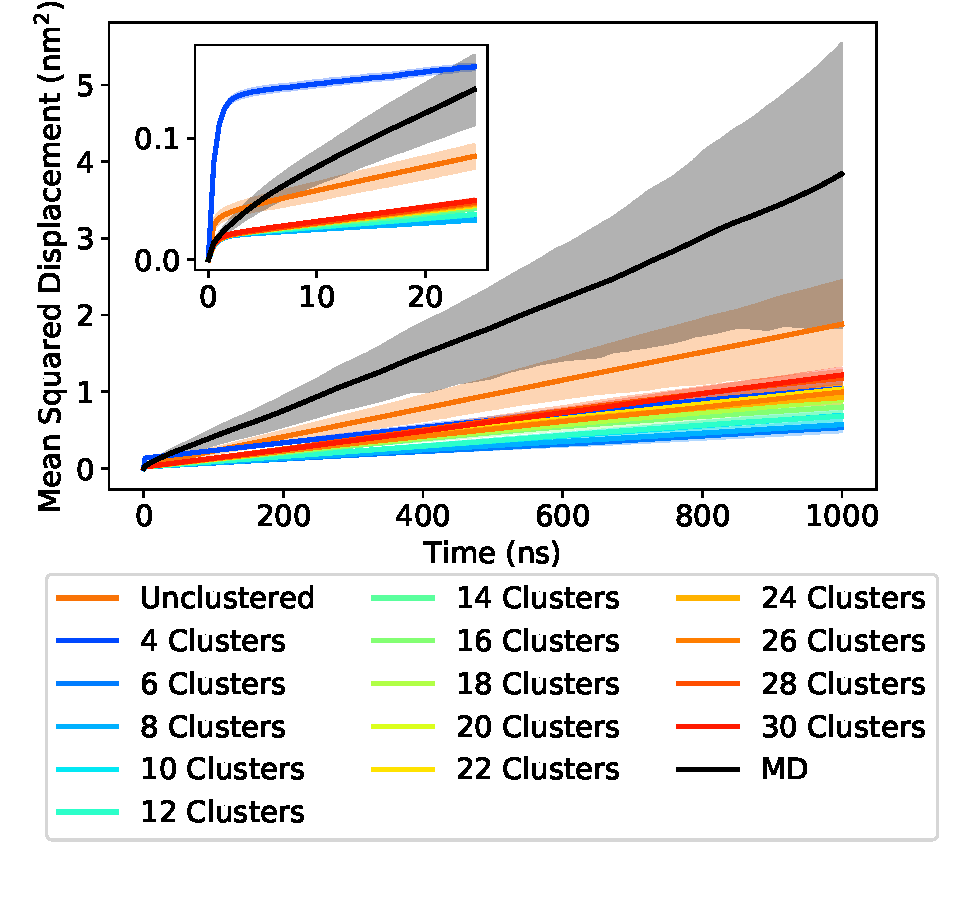
\includegraphics[width=\textwidth]{nclusters_msd_MET_complete.pdf}
%  \caption{complete}\label{fig:nclusters_msd_MET_complete}
%  \end{subfigure}
%  \begin{subfigure}{0.475\textwidth}
%  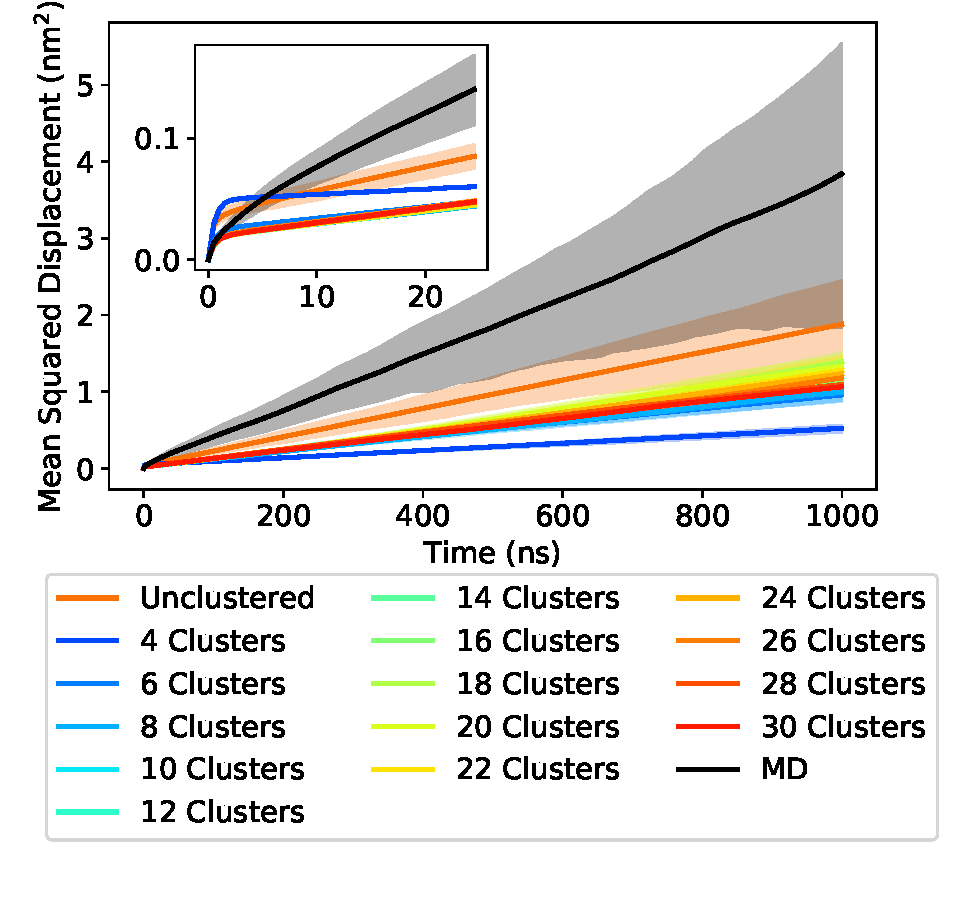
\includegraphics[width=\textwidth]{nclusters_msd_MET_average.pdf}
%  \caption{average}\label{fig:nclusters_msd_MET_average}
%  \end{subfigure}
%  \begin{subfigure}{0.475\textwidth}
%  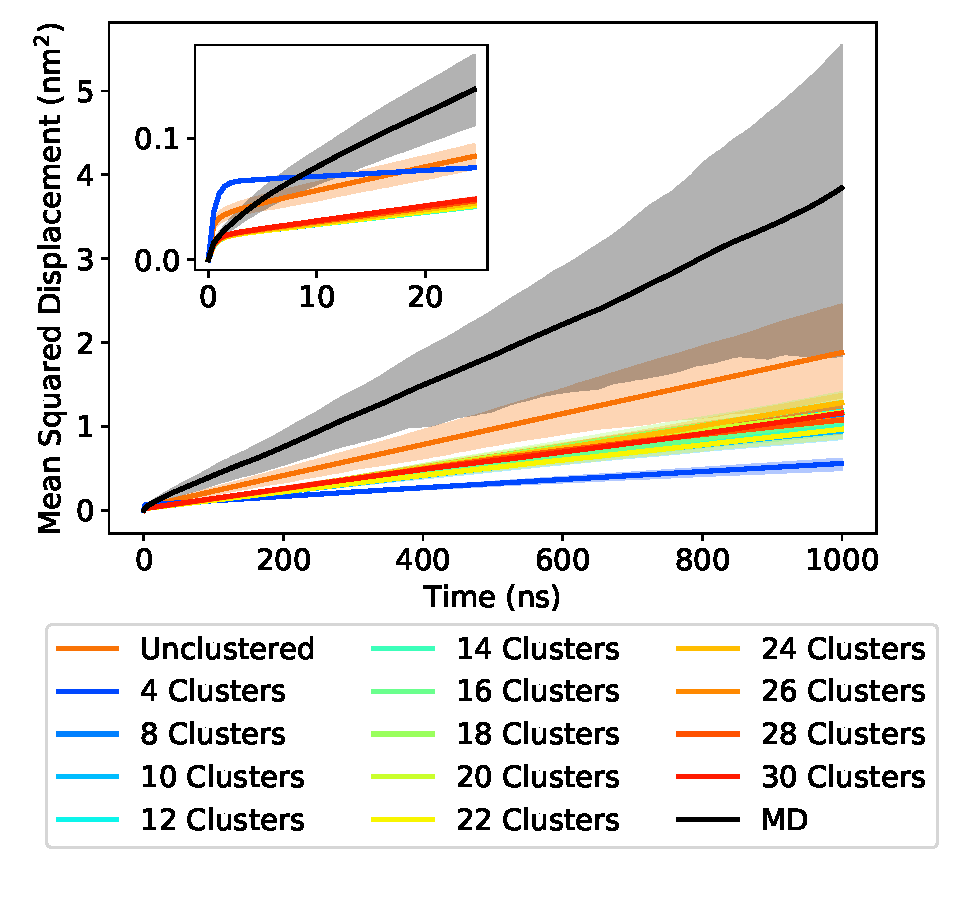
\includegraphics[width=\textwidth]{nclusters_msd_MET_single.pdf}
%  \caption{single}\label{fig:nclusters_msd_MET_single}
%  \end{subfigure} 
%  \caption{}\label{fig:MET_nclusters} 
%  \end{figure}
  

  \section{Deviations of the IHMM from Molecular Motion}\label{section:shorttimes_msd}
  
   At extremely short time lags, the MSD is generally over-predicted by the IHMM
  (see Figure~\ref{fig:unclustered_msd_shortlag}) because the VAR(1) model assumes
  multivariate Gaussian noise while the MD data suggests the noise is better 
  modeled by more general L\'evy stable noise. The first time lag of the MSD is
  equivalent to the variance of all observed fluctuations (first-order difference). 
  The IHMM simulation appears to over-estimate the variance because the actual 
  distribution of solute fluctuations has heavy tails with a smaller variance (Figure~\ref{fig:emission_widths}).
  The total distribution of hops is expected to be heavy tailed because it is a
  combination of hop distributions from many states with different variances. More
  interestingly, in Figure ~\ref{fig:state_emission_widths}, we show that the 
  emission distribution of a single state picked out by the IHMM is fit better by
  a more general L\'evy distribution while the emissions from IHMM realizations are
  Gaussian, as expected. An improvement to the IHMM that may allow dynamics more 
  faithful to MD would use an autoregressive model with L\'evy stable noise. However,
  this would be less computationally efficient due to lack of conjugate priors.
  
  \begin{figure}
  \centering
  \begin{subfigure}{0.32\textwidth}
  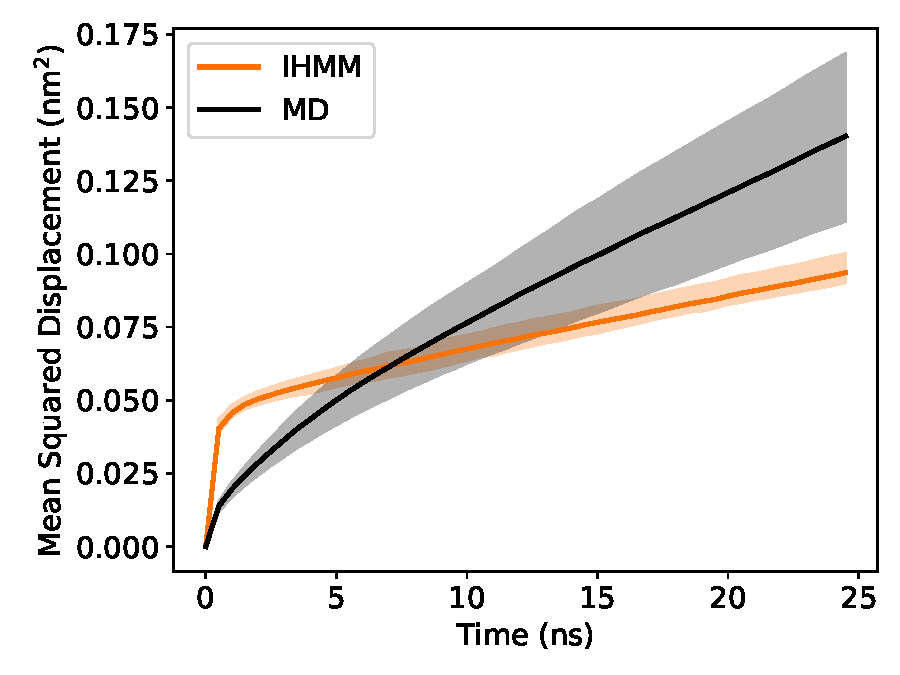
\includegraphics[width=\textwidth]{unclustered_msd_MET_shortlag.pdf}
  \caption{}\label{fig:unclustered_msd_shortlag}
  \end{subfigure}
  \begin{subfigure}{0.32\textwidth}
  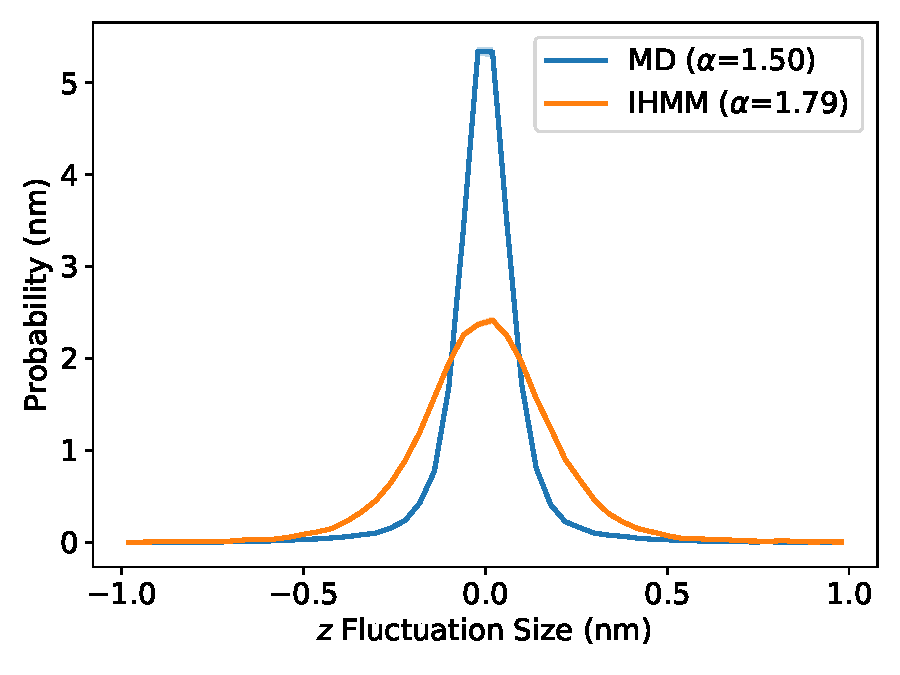
\includegraphics[width=\textwidth]{emission_widths.pdf}
  \caption{}\label{fig:emission_widths}
  \end{subfigure}
  \begin{subfigure}{0.32\textwidth}
  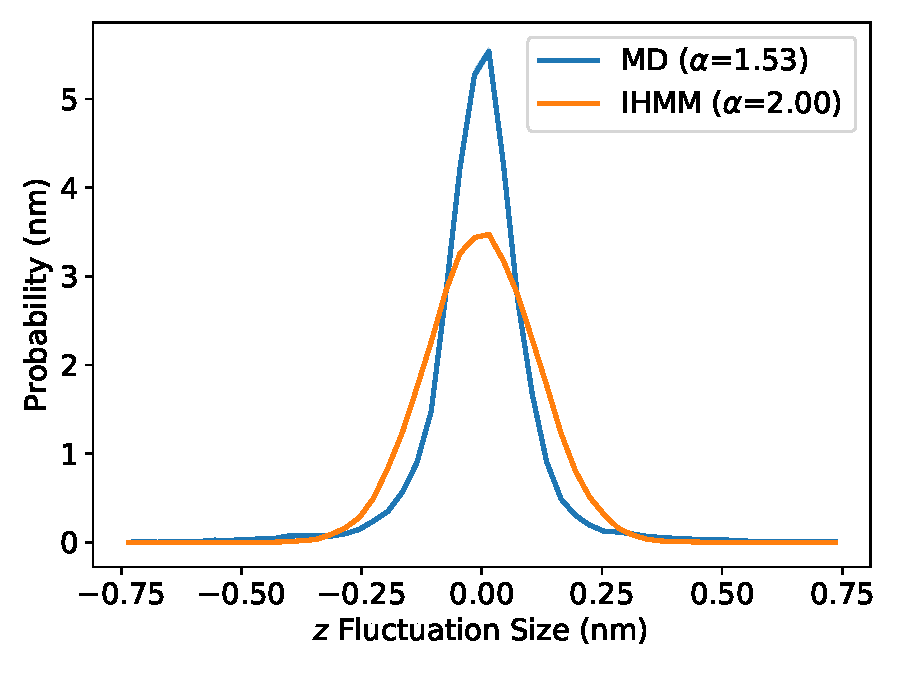
\includegraphics[width=\textwidth]{state_emission_widths.pdf}
  \caption{}\label{fig:state_emission_widths}
  \end{subfigure}
  \caption{(a) At short time lags, the MD MSD (black) and the IHMM MSD (orange)
  differ significantly in their shape and curvature. (b) While the 
  fluctuations in $z$ of both distributions are heavy-tailed, fitting well to zero-centered
  symmetric L\'evy stable distributions with stability parameters, $\alpha$, the IHMM has
  a wider variance. (c) The distribution of fluctuations in a chosen state frequently
  visited by methanol is heavy tailed, but the IHMM is constrained to produce fluctuations
  from a multivariate normal distribution ($\alpha$=2 in each dimension).
  }\label{fig:short_timelags}
  \end{figure}
  
  Also apparent from Figure~\ref{fig:unclustered_msd_shortlag} is that the 
  curvature of the MD MSD is far more gradual than that generated by the IHMM.
  This is because the VAR(1) model is only correlated to its previous fluctuation
  while the MD simulations suggest that correlation persists for at least tens
  of nanoseconds.
    % BJC2: could probably use a correlation function to suggest the AR order and stick the plot in SI
  One may be able to reproduce the curvature at short time lags with higher order
  VAR models, but it becomes a much higher dimensional parameterization that would
  require significantly more data in order to produce stable results. Since we 
  are interested in reproducing longer time scale behavior, it is not an issue of
  great concern.
  
  \section{Influence of number of clusters on qualitative hybrid trajectories}
  
  \begin{figure}
  \begin{subfigure}{0.48\textwidth}
  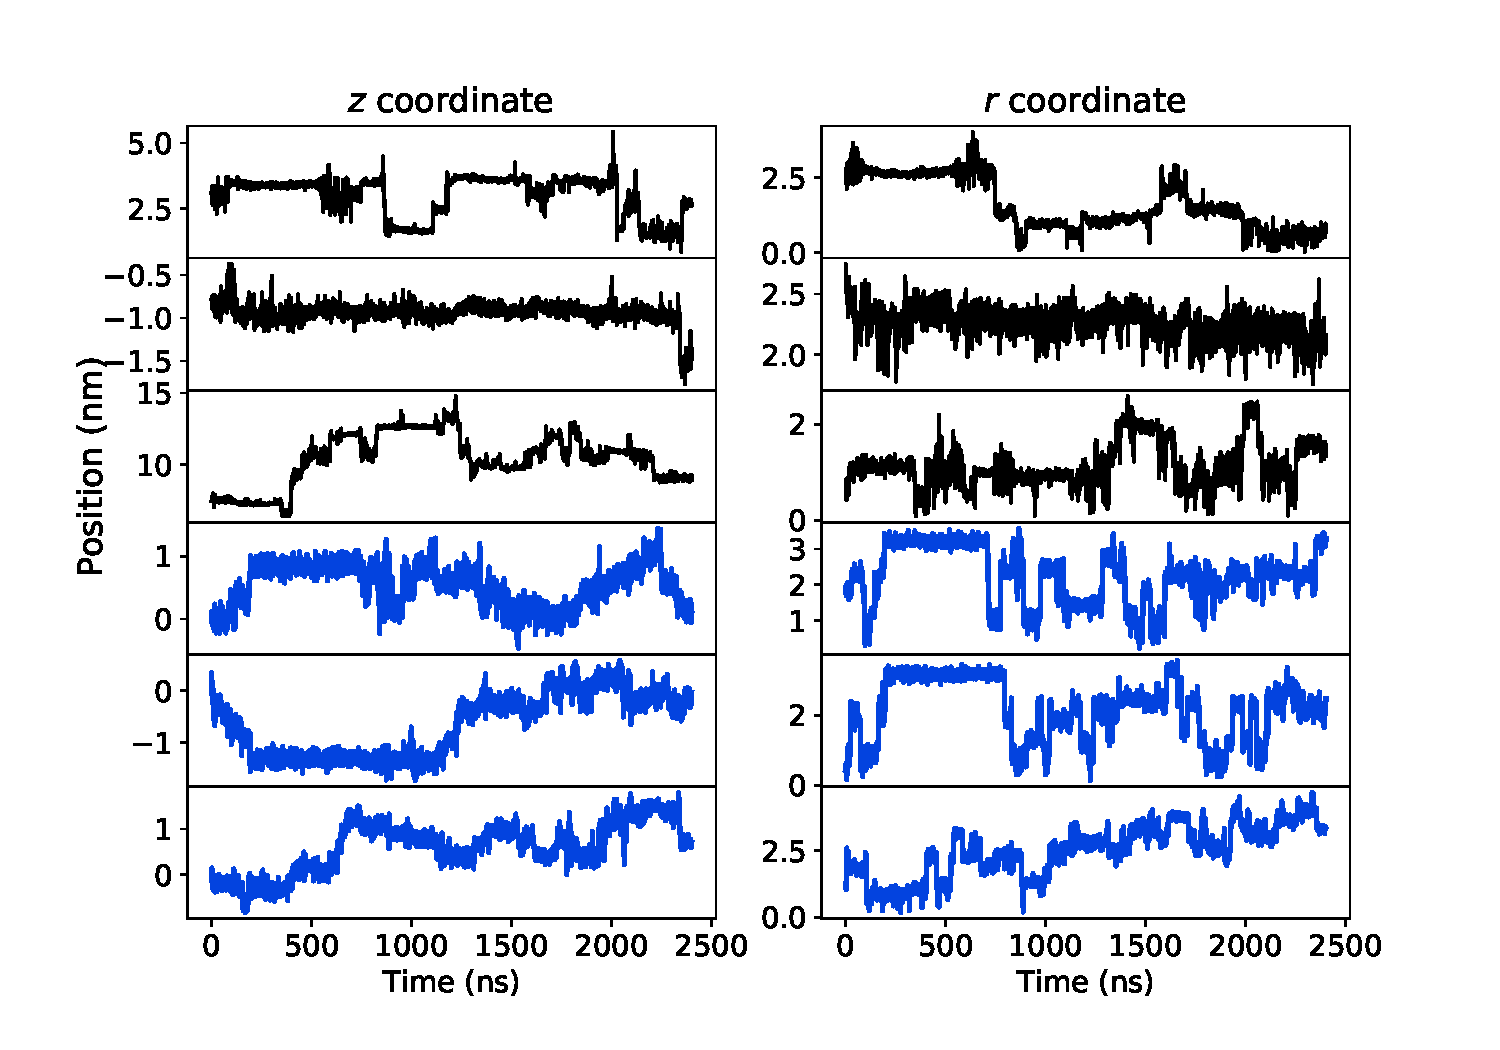
\includegraphics[width=\textwidth]{qualitative_clustered_MET_20.pdf}
  \caption{20 clusters}\label{fig:qualitative_20}
  \end{subfigure}
  \begin{subfigure}{0.48\textwidth}
  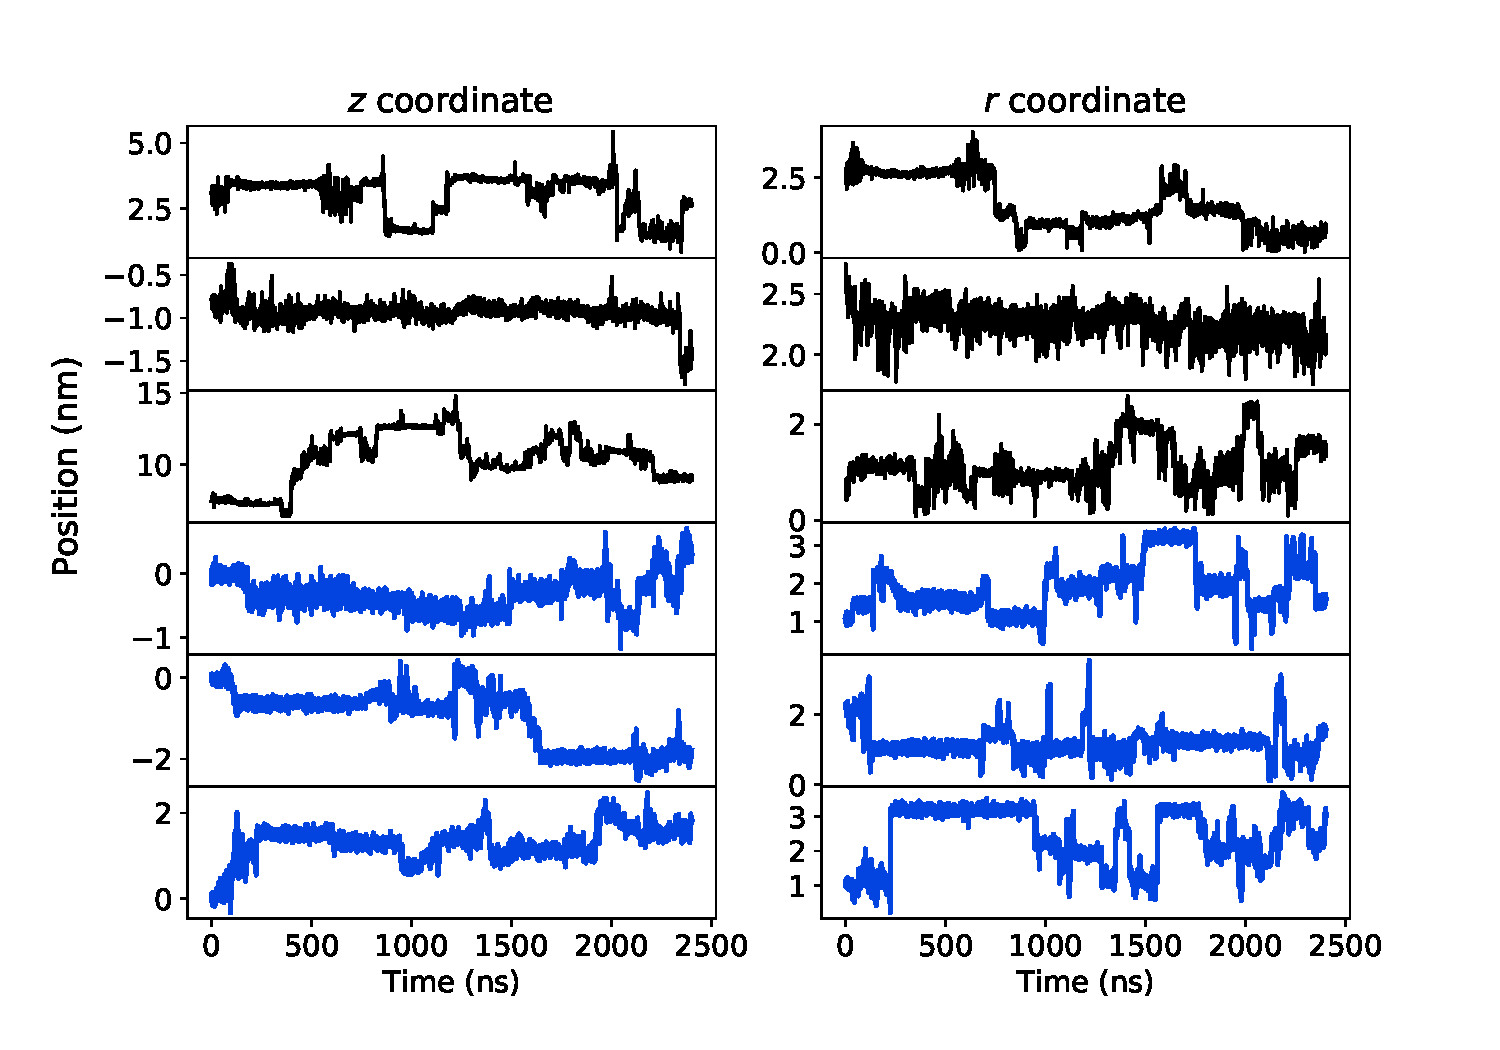
\includegraphics[width=\textwidth]{qualitative_clustered_MET_30.pdf}
  \caption{30 clusters}\label{fig:qualitative_30}
  \end{subfigure}
  \caption{The quality of hybrid trajectories resulting from clustered parameters
  sets qualitatively improves as the number of clusters is increased. This comes 
  at the cost of a larger state space to interpret.}\label{fig:qualitative_improvement}
  \end{figure}
  
  \section{Clustered Parameters}\label{section:clustered_parmeters}
  
  We can begin to hypothesize mechanisms by studying the behaviors defined by the 
  state parameters. In Figure~\ref{fig:common_states_lines}, we plot representative 
  dynamics of each of the five most visited states (see Figure~\ref{M-fig:prevalence}
  of the main text). The states exhibit a range of autoregressive and trapping 
  behavior throughout the membrane pores.
  
  Since the radial means are weighted averages of the states used to parameterize
  each cluster, for interpretive purposes, it is important to recognize that the means
  only provide clues towards the general location of the solute. For example, the 
  radial mean of state 3 is 1.4 nm from the pore center. However, inspection of 
  Figure~\ref{fig:clustered_traj_MET} suggests that this type of behavior actually
  occurs radially throughout the pore. There are instances of state 3 less than 1 nm
  from the pore center and more than 2 nm from the pore center. In this case, the 
  radial mean only suggests that this type of behavior happens in both regions somewhat
  equally.
  
  Solutes exhibit a range of autoregressive behavior as shown by the representative 
  solute trajectories in Figure~\ref{fig:common_states_lines} and the scatter
  plot in Figure~\ref{fig:A_sigma_scatter}. In most cases, the eigenvalues of $A$ and
  $\Sigma$ appear nearly paired in their radial and axial dimensions, which implies 
  nearly symmetric behavior with off-diagonals both matrices near zero. The most 
  notable exception is state 3, which has a much higher radial eigenvalue of the 
  covariance matrix. Both eigenvalues of state 3's covariance are actually quite
  large. This implies relatively large fluctuations in the $z$ direction and even
  bigger fluctuations in the $r$ direction. All states have slightly lower covariance
  in the axial direction. It's likely easier for solutes to move laterally rather 
  than to move up through the alkane chains. States 3 and 4 show a strong previous-hop
  dependence (high $A$) while the rest of the states have a somewhat weaker dependence.

  Solutes stay trapped for various lengths of time. On average, state 4 has the longest 
  dwell times and state 3 has the shortest dwell times while the rest have intermediate
  dwell times. This is somewhat supported by inspection of Figure~\ref{fig:clustered_traj_MET},
  however. The expected dwell times of the clusters incorporate all 24 trajectories.
  
  % BJC4: Not sure if this is useful.
  % MRS: it does give a good summary. But you should make it clear how you selected these 5.
  % MRS: it's implied in one of the figures, but should be stated explicitly
%  By examining the parameters, it is now easier to describe the state behavior.
%  \begin{enumerate}[label={State \theenumi :}, leftmargin=3.5\parindent]
%     \item This state has intermediate dwell times with high past-hop dependence.
%     The radial mean and evidence from Figure~\ref{fig:clustered_traj_MET} suggests
%     %MRS: ``tail and pore region'' sounds the same as ``everywhere''.
%     that this state is common in the tail and pore region.
%     \item This state seems to occur exclusively in the tail region based on its radial
%     mean. Its fluctuations are small and there is little past hop dependence
%     \item This is likely a hopping state that strongly contribute to the solute's MSD. 
%     It is short lived and takes very large hops. This type of behavior is exhibited 
%     %MRS: ``near and far'' also sounds like everywhere 
%     near and far from the pore center as discussed earlier.
%     \item This is a trapping state with a strong dependence on its previous fluctuation.
%     Evidence from Figure~\ref{fig:clustered_traj_MET} and a radial mean of 1.8 suggest
%     that it tends to occur at intermediate distances from the pore center.
%     \item This is an intermediate-length trapping state that occurs close to the pore
%     center. It's fluctuations are tight and relatively independent of its previous 
%     fluctuation.
%  \end{enumerate}  
  
  \begin{figure}
  \centering
  \begin{subfigure}{0.58\textwidth}
  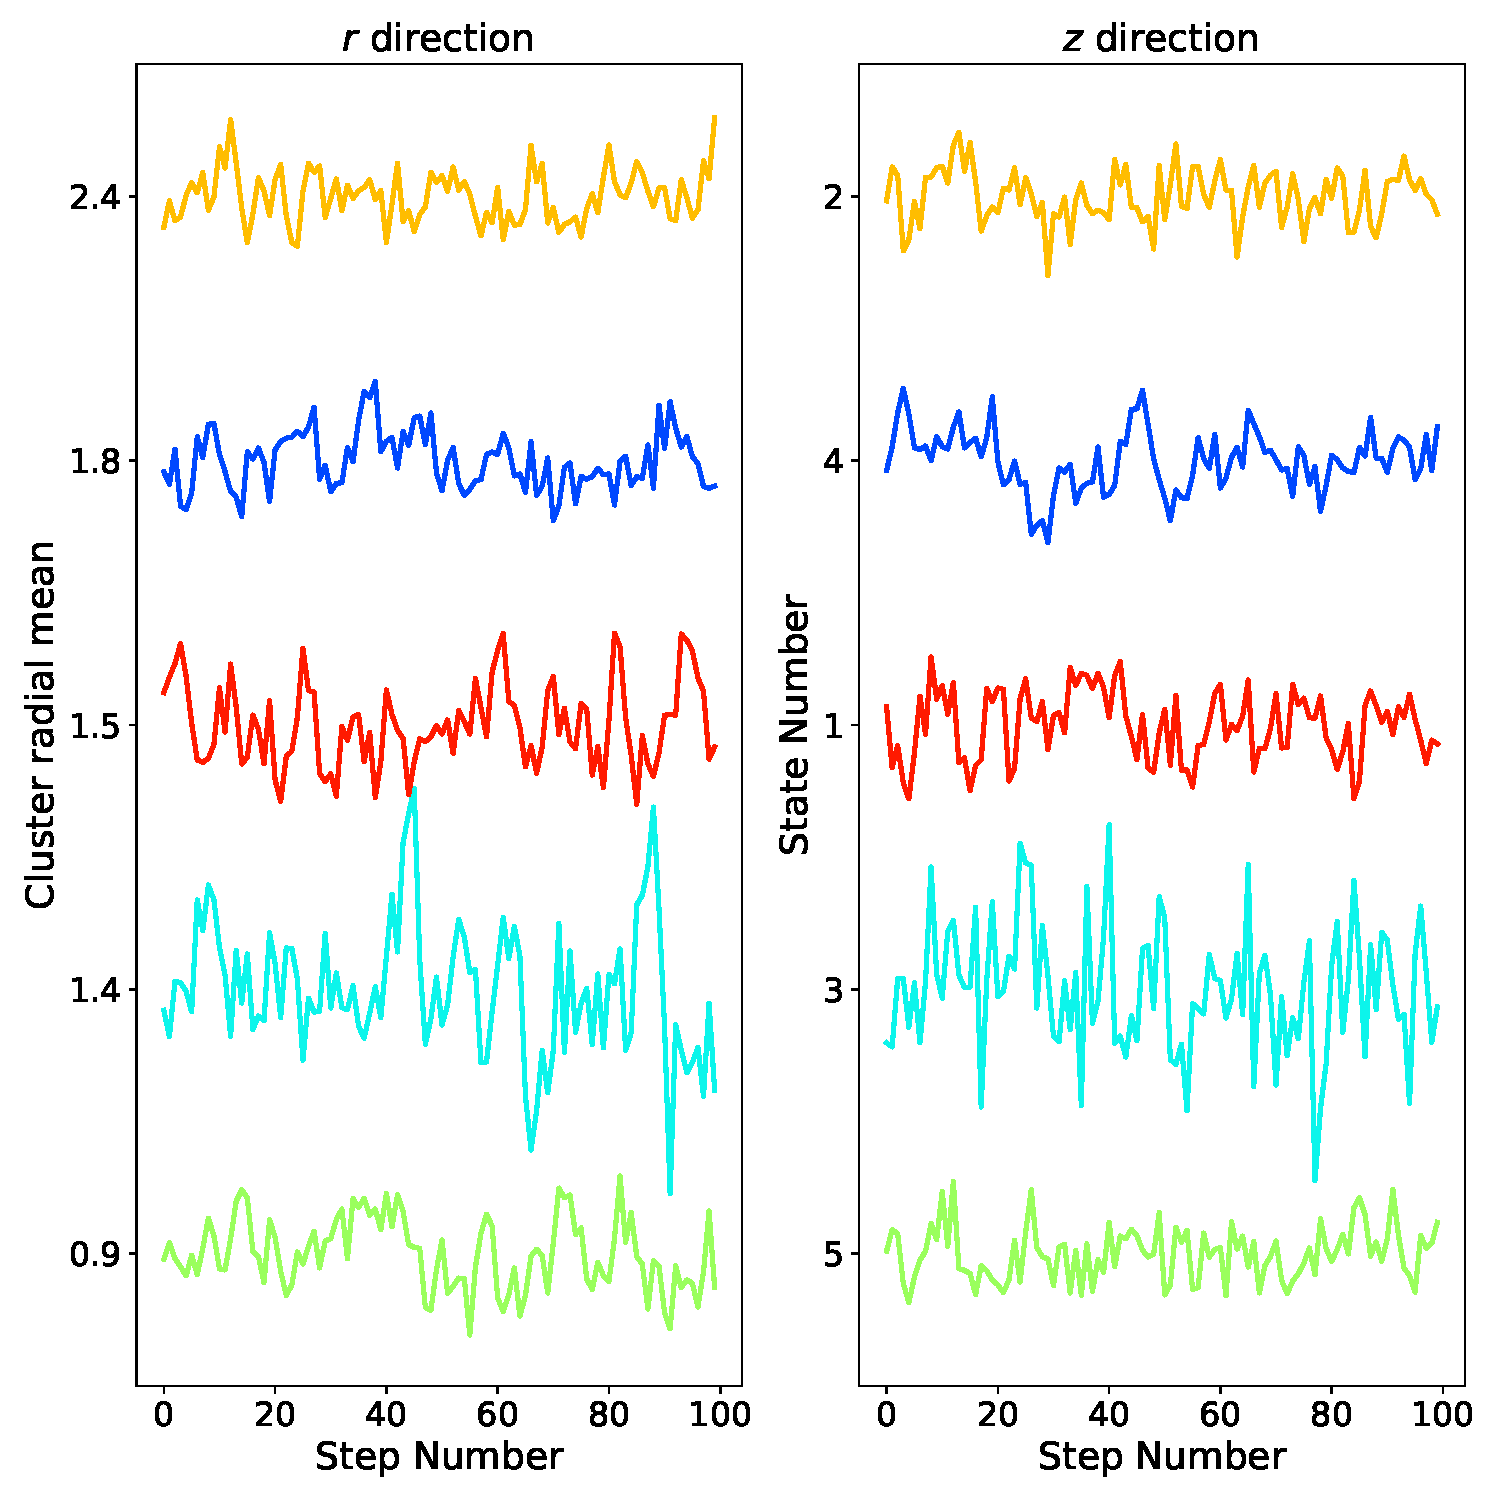
\includegraphics[width=\textwidth]{common_states.pdf}
  \caption{}\label{fig:common_states_lines}
  \end{subfigure}
  \begin{subfigure}{0.41\textwidth}
  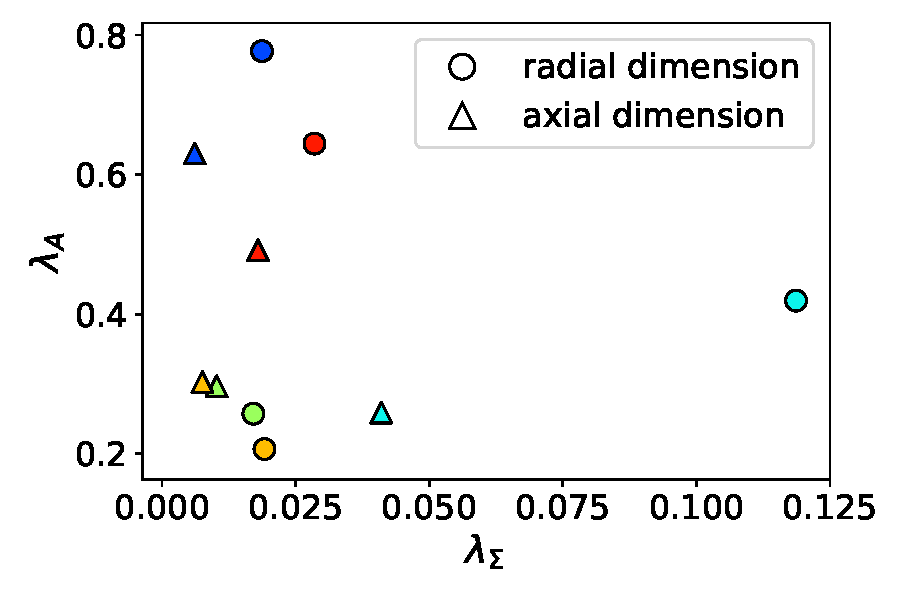
\includegraphics[width=\textwidth]{A_sigma_scatter.pdf}
  \caption{}\label{fig:A_sigma_scatter}
  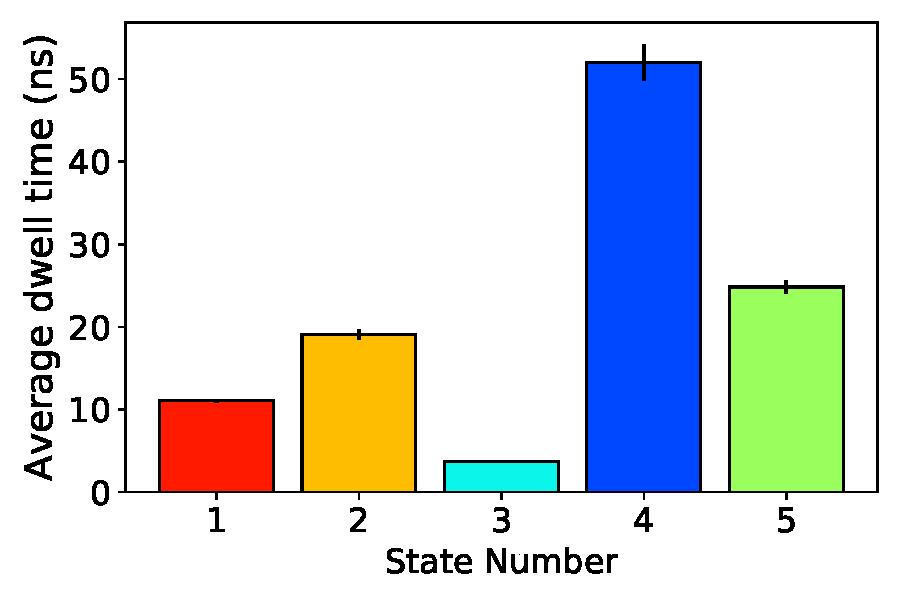
\includegraphics[width=\textwidth]{dwell_times.pdf}
  \caption{}\label{fig:dwell_times}
  \end{subfigure}
  \caption{The 5 most visited states by methanol show a range of dynamical behavior. In 
  (a), we show representative dynamics of these states. All time series have a mean of zero and are
  shifted to put the mean in line with the $y$-axis labels for the purpose of visualizing them.
  The $y$-axis labels of the $r$ coordinate plot specify the radial mean of each clustered 
  state. All of the states pictured appear in the trajectory shown in 
  Figure~\ref{M-fig:clustered_traj_MET} of the main text and are colored to match.
  (b) We can begin to understand the solute behaviors demonstrated in (a) by understanding their VAR 
  parameters. Higher values of $\lambda_{\Sigma}$ generally are indicative of large fluctuations
  and higher values of $\lambda_A$ indicate strong previous-hop dependence of the fluctuations.
  (c) Using Equation~\ref{M-eqn:dwell_times} of the main text, we estimated the expected time spent within each 
  of the states.
  }\label{fig:common_states_MET}
  \end{figure}
  
  The local number density of heavy atoms surrounding solutes help round out methanol's
  mechanistic picture. Although hydrogen bonding interactions are relatively frequent,
  methanol molecules are unbound by any measurable electrostatic interactions about 
  half or more of the simulation time. Figure~\ref{fig:local_densities} helps to 
  illustrate how the local density of membrane components can aid in solute entrapment.
  When solutes experience long trapping times, the local number density of heavy atoms
  is larger. Even when hydrogen bonds break, surrounding alkane density likely helps 
  keep the solutes in place allowing them to eventually reform. This can happen deep 
  in the tails or close to the monomer head groups. Methanol molecules which experience
  State 3 have by far the smallest local number density which is likely responsible for 
  their mobility, as suggested by the state's large covariance.
  
  \begin{figure}
  \centering
  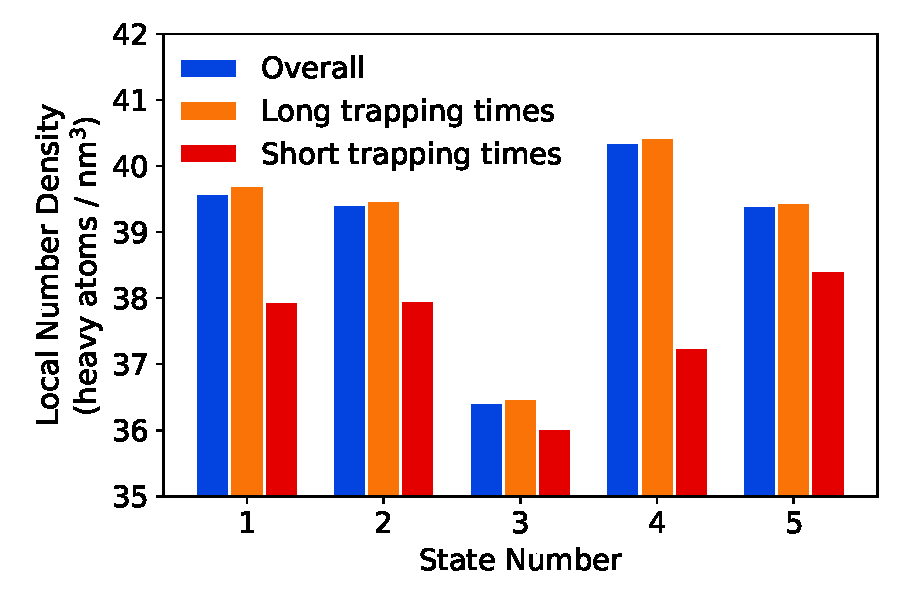
\includegraphics[width=0.5\textwidth]{local_densities.pdf}
  \caption{We measured the local number density of heavy atoms surrounding solutes in each
  state. In blue, we plot the local number density experienced by solutes averaged over all
  frames in which the solute occupied the given state. We broke down this overall average 
  number density into number densities measured from instances when the state is occupied 
  for long (orange) versus short(red) dwell time states. We define define `long' dwells times
  as the 50th percentile of all dwell times in the given state, and short as all others. It
  is clear that solutes which experience longer dwells times are also surrounded by more 
  heavy atoms on average.}\label{fig:local_densities}
  \end{figure}
  
\end{document}